%!TEX program = XeLaTeX
%!TEX encoding = UTF-8 Unicode

%%%%%%%%%%%%%%%%%%%% book.tex %%%%%%%%%%%%%%%%%%%%%%%%%%%%%
%
% sample root file for the chapters of your "monograph"
%
% Use this file as a template for your own input.
%
%%%%%%%%%%%%%%%% Springer-Verlag %%%%%%%%%%%%%%%%%%%%%%%%%%


\documentclass[graybox,envcountchap,sectrefs]{svmono}

% choose options for [] as required from the list
% in the Reference Guide

\usepackage{mathptmx}
\usepackage{helvet}
\usepackage{courier}
%
\usepackage{type1cm}

\usepackage{makeidx}         % allows index generation
\usepackage{graphicx}        % standard LaTeX graphics tool
                             % when including figure files
\usepackage{multicol}        % used for the two-column index
\usepackage[bottom]{footmisc}% places footnotes at page bottom
\usepackage[numbers]{natbib}

% support Chinese
%\usepackage{CTex}
%\usepackage{ctex}
\usepackage[UTF8]{ctex}

\usepackage{amsmath,bm}
\usepackage{amssymb}
\usepackage{color}
\usepackage{graphicx}
%\usepackage[unicode]{hyperref}
\usepackage{xcolor}
\usepackage{indentfirst}
\usepackage{enumerate}
%\usepackage{epstopdf}
%\usepackage{titlesec}
\usepackage{mathrsfs}
\usepackage[ruled,linesnumbered]{algorithm2e}
\usepackage{epsfig,tabularx,amssymb,amsmath,subfigure,multirow,graphicx}
%\usepackage{fontspec}
\usepackage{diagbox}
\usepackage{longtable}
\usepackage{hyperref}

% see the list of further useful packages
% in the Reference Guide

\makeindex             % used for the subject index
                       % please use the style svind.ist with
                       % your makeindex program

%%%%%%%%%%%%%%%%%%%%%%%%%%%%%%%%%%%%%%%%%%%%%%%%%%%%%%%%%%%%%%%%%%%%%

\begin{document}

%\author{CSLT}
\title{自然语言处理与生物识别}
\subtitle{Natural Language Processing for Biometric Identification}
\maketitle


\frontmatter%%%%%%%%%%%%%%%%%%%%%%%%%%%%%%%%%%%%%%%%%%%%%%%%%%%%%%

%\include{dedic}
%\include{foreword}
%\include{preface}
%\include{acknow}

\tableofcontents

%\include{acronym}

\mainmatter%%%%%%%%%%%%%%%%%%%%%%%%%%%%%%%%%%%%%%%%%%%%%%%%%%%%%%%
%%%%%%%%%%%%%%%%%%%%% chapter.tex %%%%%%%%%%%%%%%%%%%%%%%%%%%%%%%%%
%
% sample chapter
%
% Use this file as a template for your own input.
%
%%%%%%%%%%%%%%%%%%%%%%%% Springer-Verlag %%%%%%%%%%%%%%%%%%%%%%%%%%
%\motto{Use the template \emph{chapter.tex} to style the various elements of your chapter content.}
\chapter{NLP发展现状与应用领域}
\label{basic} % Always give a unique label
% use \chaptermark{}
% to alter or adjust the chapter heading in the running head

\section{定义简介}
自然语言处理(Natural Language Processing,简称NLP),属于计算机科学与语言学的交叉学科,所以又称计算语言学;它是用计算机来理解、处理、运用人类语言的学科。人类通过自然语言进行沟通协作,可以说如果没有语言人类的智能将无从谈起,它是人类区别于动物的重要标志。也可以说,只有当计算机具备了准确的自然语言的理解处理能力时,才算真正实现了人工智能。
\begin{itemize}
\item 研究内容:NLP研究内容主要包括词法分析、句法分析、语义分析、篇章理解、机器翻译等。
\item 应用场景:NLP广泛应用信息系统方方面面。例如:手写体识别、光学符号识别、语音识别、语音合成、信息检索、机器翻译、对话系统等。
\item 关联学科:NLP紧密相关的研究领域包括机器学习、数据挖掘、知识图谱等;紧密相关的学科包括信息论、语言学、计算机科学等。
\end{itemize}

NLP研究范围涉及自然语言的形态学、语法学、语义学和语用学等几个层次。
\begin{itemize}
\item 形态学(morphology):研究词的内部结构,包括屈折变化和构词法两个部分。
\item 语法学(syntax):研究句子结构成分之间的相互关系、句子序列的组成规则。
\item 语义学(semantics):研究各级语言单位(词素、词组、句子、段落、片等)的意义,以及与语音、语法、语境的关系等等,其重点在探明符号与其所指对象之间的关系。
\item 语用学(pragmatics):研究在不同上下文下的语句应用,以及上下文对语句理解所产生的影响。大概来说,语用学研究范围问题是很广,重点在于研究包括直指、会话隐含、预设、语言行为、话语结构等。
\end{itemize}

NLP面临的两大难题是歧义消解、未知语言现象。
\begin{itemize}
\item 歧义消解:在自然语言的词法、句法、语义等各个层次中存在大量的歧义现象。比如“什么是一个词”,这就是NLP面临的一个难题。因为不同的人对词语粒度、标准有不同的理解。再比如,语言中存在大量一词多义的现象,在上下文语境中如何准确找到对应的词义,这些都是NLP研究面临的实实在在的难题。
\item 未知语言现象:未知语言现象主要由两个方面的原因导致。第一点,人类语言一直处于不断演化过程中,同一个语言表达,在新的时空环境下,可能已经不再是以前的含义;而且,由于信息网络的发达,人们构造、传播新语言现象的能力大大增强,比如互联网上每天都在涌现新的语言词汇。第二点,在NLP研究中,由于整理收录能力、知识表达能力等现实因素的制约,实际中并没有一种可以准确、全面表达人类语言知识工程或工具。
\end{itemize}

\section{发展历史}
NLP发展历史中存在两种不同的的研究方法:基于规则的理性主义;基于统计的经验主义。它们对语言的不同理解,体现了它们不同的哲学思想。
\begin{itemize}
\item 理性主义:认为自然语言是由语言规则来产生和描述的;因此他们相信,只要能够用适当的形式将人类语言规则表示出来,就能够理解人类语言。
\item 经验主义:认为语言知识可以从语言数据中获取,只要建立有效的统计模型就可以理解语言;因此他们相信,如果有足够多语言数据用于统计,就能够理解人类语言。
\end{itemize}

NLP发展历史可以总结为5个时期:
\begin{enumerate}
\item 经验主义萌芽时期:时间大约到20世纪50年代。这个时期NLP或多或少具有经验主义色彩。例如,1913年马尔科夫提出马尔科夫模型\cite{markov1913example}的时候,就曾经计算过长诗中元音与辅音出现的频度概率;再比如,1948年,香农把离散马尔科夫的概率模型应用于语言自动机\cite{shannon1948mathematical}的时候,也曾统计过英语字母的频率。

\item 经验主义低谷时期:时间从1956年~20世纪90年代。1956年,乔姆斯基首先提出使用有限状态机来刻画自然语言\cite{chomsky1956three}。具体来说,就是使用数学的代数、集合论为基础核心,将各种语言现象统一抽象为代数、集合上的运算规则。形式语言理论影响深远,在此后很长一段时期,很多学者逐步完善并扩展了形式语言理论。这段时期,NLP领域的研究方法几乎完全被理性主义主导,经验主义被打入谷底。

\item 经验主义复苏时期:时间从20世纪50年代末到90年代初期。虽然这期间,例行理性主义占据主流,但是有学者已经开始思考引入基于语料库的统计方法到NLP研究中;这其中的代表是1967年诞生的联机语料库Brown Corpus\cite{kuvcera1967computational}。另外,和NLP紧密相关的机器学习方法得到了较大的发展;比如这段时期,诞生了贝叶斯模型、最大熵\cite{jaynes1957information}、维特比算法\cite{viterbi1967error}、隐马尔可夫模型\cite{stratonovich1965conditional}等等,NLP研究有了更多理论工具可供使用。

\item 经验主义爆发时期:时间20世纪90年代中期~2010年左右。时间处于20世纪90年代前期,此刻经验主义已经处于全面复苏的前夜。一方面,由于机器学习领域诞生了很多新理论和方法,推动了NLP快速发展;另一方面,计算机的存储容量、计算能力已经极大提升,使得很多计算量偏大的机器学习方法逐渐实用。受益于这两方面,经验主义终于开始全面复苏,迎来了一个前所未有的黄金时期。20世纪90年代以后,以语料库和统计学习为基础,基于机器学习的词法分析、句法分析、机器翻译、语音识别等研究不断涌现。Ruder\cite{ruder2018review}在文章中总结了此时期,一些影响力较大里程碑,按照时间线索列举如下:

\begin{itemize}
    \item 1993年,IBM提出了基于语料库的统计机器翻译模型\cite{brown1993mathematics},吹响了经验主义的全面复苏的号角。
    \item 1994年,隐马尔科夫模型在语音识别\cite{lee1989speaker}\cite{deng1994speech}中成功运用,标志了经验主义全面复苏。
    \item 1998年,Berkeley大学主导了FrameNet项目\cite{baker1998berkeley},提出了框架语义学并开放了语料库。这个项目,大大提升了语义角色标注的效果,并在后续促进了,组块分析、依存分析等其他NLP任务的发展。
    \item 2001年,Lafferty发表了条件随机场(Conditional Random Fields,CRF)\cite{lafferty2001conditional}模型。从此,CRF成为序列标注任务的标志性模型,被广泛用于自动分词、词性标注、专名识别等NLP任务中。
    \item 2002年,IBM提出了BLEU\cite{papineni2002bleu},给出了双语互译质量度量的自动评估标准,结束了翻译效果人工评估繁重主观的难题,为后续机器翻译快速发展奠定基础。同年,结构化感知机\cite{collins2002discriminative}的出现,丰富了序列标注方法,很快也被广泛应用序列标注任务中。另外,情感分析\cite{pang2002thumbs}也开始成为NLP研究热点之一。
    \item 2003年,诞生了用于主题建模的标准模型LDA\cite{blei2003latent}(Latent Dirichlet Allocation),它被应用于主题建模、文本分类、相似度计算等方面。
    \item 2004年,Taskar等人提出最大边缘模型\cite{taskar2004max},相比于SVM,它更适合获取结构化数据中的相关性,应用于句法解析任务中。
    \item 2006年,Hovy等人发布大型多语言语料库OntoNotes\cite{hovy2006ontonotes},它已被用于训练、评估多个NLP任务,如专名识别、依存分析等。
    \item 2008年,Milne等人介绍了利用维基百科计算语义相关性\cite{witten2008effective}的方法。维基百科,到目前为止,依旧是NLP语料库最重要成员之一,被广泛用于语言模型、实体链指、知识图谱等各种NLP任务。
    \item 2009年,Go等人提出了远程监督(Distant Supervision)\cite{go2009twitter}的思想,利用维基百科丰富了情感分类标注数据,获得任务效果的较大提升。此后,远程监督思想被更多学者,扩充到关系抽取、信息抽取、情感分类、文本分类等NLP任务中。它们大多通过利用现有大型知识库、语料库(比如维基百科),通过启发式方法,从中抽取大量带有噪声的数据,用于弥补标注数据的不足。
\end{itemize}

\item 经验主义现代时期:时间从2003年左右至今。这段时期,经验主义再上高峰,具有更加鲜明的特色,神经网络、深度学习的是目前NLP研究的关键词。Ruder在博文\cite{ruder2018review}在中总结了这段时期里NLP的研究趋势,归结为8个方面,列举如下:

\begin{itemize}
    \item 神经语言模型(Nerual Language Model,NLM):语言模型是NLP中基础工具,它处理的是给定上文,建模下一个词出现的概率。2003年,Bengio等人提出基于神经网络的语言模型\cite{bengio2003neural},用于替代传统基于计数和平滑的ngram语言模型。此后,NLM被众多研究者进行了扩展,出现了基于标准循环神经网络(RNN)、\cite{mikolov2010recurrent}、长短时记忆网络(LSTM)\cite{graves2013generating}等变种。
    \item 多任务学习(Multi-task Learning):多任务学习通过共享模型参数,使得多个任务可以协同学习、共同提升。2008年,Collobert等首次将多任务学习\cite{collobert2008unified}应用于NLP。到现在,多任务学习在NLP任务中广泛体现,并且很多学者还在不断发展和扩充此思想。
    \item 词嵌入(Word Embedding):在NLP和信息检索领域,人们为了表示一个句子的含义,常常忽略句子的文法和语序,仅考虑频次,采用One-Hot编码,简化成词袋(Bag Of Words)模型进行表达。One-Hot编码有两个缺陷:1. 编码向量高维稀疏;2.不方便计算词之间的相似度。2013年,Mikolov等人提出了词嵌入模型word2vec\cite{mikolov2013efficient},改用低维稠密向量对词语进行编码,获取的词向量蕴含了语言中的近义、同位、上下位等性质。由于词向量蕴含的语义相似度特性,它已成为NLP在深度学习时代的标配,在后续的研究中发挥了重要作用。
    \item NLP神经网络(Neural Networks For NLP):2013年,神经网络开始应用于NLP任务。2013年,Graves等将循环神经网络\cite{graves2013hybrid}应用于语音识别;2013年,Socher等使用递归神经网络\cite{socher2013recursive},改进了传统的句法分析;2014年,Kalchbrenner\cite{kalchbrenner2014convolutional}等人和Kim\cite{kim2014convolutional}等人,将卷积神经网络用于句子建模和文本分类。至此,神经网络3大结构,都成功应用于NLP中。
    \item Seq2Seq(Sequence To Sequence Model)模型:它是将一个序列映射到另一个序列的通用框架,包含编码器和解码器两部分。编码器将输入句子,压缩为一个固定大小的向量;解码器根据前一步输出和当前状态预测当前位置的输出。2014年,Sutskever等人首次提出了Seq2Seq\cite{sutskever2014sequence}模型框架,将其成功应用于机器翻译任务。它标记着机器翻译,从此进入神经网络机器翻译(Nerual Machine Translation,NMT)时代。后续,很多研究扩展了Seq2Seq的应用范围,产生了比如图像标题生成,文本生成等有趣的应用。
    \item 注意力(Attention)机制:2014年,它由Bahdanau\cite{bahdanau2014neural}等人首次提出。注意力机制,是NMT又一大突破,是NMT能够超过统计机器翻译的关键;它和Seq2Seq一起,将NMT推广到大规模工业应用。通过注意力机制,解码器可以回看编码器的序列状态,极大优化了机器翻译的对齐效果,使得NMT跨进工业应用门槛。后续很多学者,提出了注意力机制的多种实现。注意力机制除了直接激发Transformer\cite{vaswani2017attention}发明,也被广泛应用句法分析\cite{vinyals2015grammar}、阅读理解\cite{hermann2015teaching}等任务。
    \item 基于记忆的网络(Memory-based Networks):由于RNN隐状态、注意力机制等提供的记忆能力不足,无法存储长期、大量的信息。所以,2015年前后,很多学者提出了基于记忆的网络来改进这一问题。其中的代表有,神经图灵机\cite{graves2014neural}、记忆网络\cite{weston2014memory}、端到端记忆网络\cite{sukhbaatar2015end}、动态记忆网络\cite{kumar2016ask}、神经微分计算机\cite{graves2016hybrid})和循环实体网络\cite{henaff2016tracking}。记忆网络技术,广泛适用于机器机器阅读理解、基于知识库的问答、多轮对话系统等方面。
    \item 预训练语言模型(Pretrained Language Models):2018年是预训练语言模型元年,因为从此以后NLP众多任务的研究范式都被改变。2018年,诞生了ELMO\cite{peters2018deep}、GPT\cite{radford2018improving}、BERT\cite{devlin2018bert}这3个杰出代表。它们通过将语言模型嵌入作为特征,使用目标任务数对语言模型对进行微调,使得众多NLP任务都获得了大幅度提升。由于预训练语言模型,只需要无标记的数据便可以进行学习,因此对于标记数据稀缺的低资源场景,预训练语言模型尤其有用。
\end{itemize}

\end{enumerate}

\section{应用领域}
自然语言处理研究的内容非常广泛,应用范围也非常广泛,如下举例一些常见的应用场景:
\begin{itemize}
\item 机器翻译:利用计算机实现自然语言(英语、汉语等)之间的自动翻译。
\item 自动摘要:利用计算机自动地从原始文档中提取全面准确地反映该文档中心内容的简单连贯的短文。
\item 文本分类:在预定义分类体系下,根据文本的特征,将给定文本于一个或多个类别相关联的过程。
\item 情感分类:根据文本所表达的含义和情感将文本划分为褒扬或者贬义的两种或几种类型,是对作者倾向性、观点、态度的划分,因此也称倾向性分析。
\item 信息抽取:从非结构化或半结构的自然语言文本中提取出于某个主题相关的实体、关系。事件等事实信息,并且形成结构化信息输出。
\item 信息检索:用户输入一个表述需求信息的查询字段,系统回复一个包含所需要信息的文档列表。其核心技术在于索引构建和相关性计算。
\item 问答系统:接受用户自然语言形式描述的问题,从大量异构数据中查找或者推断用户问题答案的信息检索系统。
\end{itemize}


%%%%%%%%%%%%%%%%%%%%% chapter.tex %%%%%%%%%%%%%%%%%%%%%%%%%%%%%%%%%
%
% sample chapter
%
% Use this file as a template for your own input.
%
%%%%%%%%%%%%%%%%%%%%%%%% Springer-Verlag %%%%%%%%%%%%%%%%%%%%%%%%%%
%\motto{Use the template \emph{chapter.tex} to style the various elements of your chapter content.}
\chapter{语言模型与主题模型}
\label{lm} 

本章简单介绍自然语言处理中的语言模型和主题模型的概念,并其常见的算法,以及在语音识别中的应用。


\section{语言模型}

\subsection{基本定义}

语言模型(Language Model)用于计算语言序列$w_1, w_2, \cdots, w_n$的概率,数学表示为$P(w_1, w_2, ..., w_n)$,它是对语句的概率分布的建模。
其最直接的应用就是判断一句话来自于人生成的语句的概率,例如在我们自然语言中,句子``我去吃饭''相比于``吃饭去我''的出现的概率更高,因此$P($``我去吃饭''$) > P($``吃饭去我''$)$。讲到这里,最直接的一个问题就是,如何计算$P(w_1, w_2, ..., w_n)$呢?我们下面介绍一种最基本的语言模型:n-gram语言模型。

\subsection{n-gram语言模型}
n-gram语言模型是一种最基础的语言模型。根据链式法则(Chain Rule),公式$P(w_1, w_2, ..., w_n)$可以得到:
\begin{equation} \nonumber
\label{equ:ab}
\begin{aligned}
P(w_1, w_2, \cdots, w_n)=P(w_1)P(w_2|w_1)\cdots P(w_n|w_1,\cdots,w_{n-1})
\end{aligned}
\end{equation}
其中的每一项$P(w_i|w_1,\cdots,w_{i-1})$,可以用以下公式来估计,即:
\begin{equation} \nonumber
\label{equ:ab}
\begin{aligned}
P(w_i|w_1,\cdots,w_{i-1}) = \frac{C(w_1,\cdots, w_{i-1}, w_i) }{C(w_1,\cdots,w_{i-1})}
\end{aligned}
\end{equation}
其中,$C(\cdot)$表示该序列在训练语料中出现的次数。但是,当序列长度很长时候,计算$P(w_i|w_1,\cdots,w_{i-1})$比较困难,一种常见的处理方式是引入马尔可夫假设(Markov Assumption),即假设当前词出现的概率只依赖于前$n-1$个词,也就是:
\begin{equation} \nonumber
\label{equ:ab}
\begin{aligned}
P(w_i|w_1,\cdots,w_{i-1}) = P(w_i|w_{i-n+1},\cdots,w_{i-1})
\end{aligned}
\end{equation}
根据$n$取值的不同,我们可以得到不同的n-gram语言模型:
\begin{itemize}
    \item Unigram: $P(w_1, \cdots, w_{i-n})=\prod_{i=1}^{n} P(w_i)$
	\item Bigram: $P(w_1, \cdots, w_{i-n})=\prod_{i=1}^{n} P(w_i|w_{i-1})$
	\item Trigram: $P(w_1, \cdots, w_{i-n})=\prod_{i=1}^{n} P(w_i|w_{i-1},w_{i-2})$
\end{itemize}

\subsection{n-gram 语言模型中的平滑技术}
在计算n-gram时候,一个很重要的问题就是测试集中出现了训练集中未出现过的词而导致语言模型计算出的概率为零,我们称这些词为未登录词(OOV)。平滑(Smoothing)技术就是为了缓解这类问题,常见的平滑技术有:拉普拉斯平滑(Laplace Smoothing),、古德图灵法(good-turing)、线性减值法(Linear Discounting)等,感兴趣的读者可以深入阅读相关论文。

\subsection{语言模型在语音识别中的应用}

\begin{figure}[h!]
	\begin{center}
		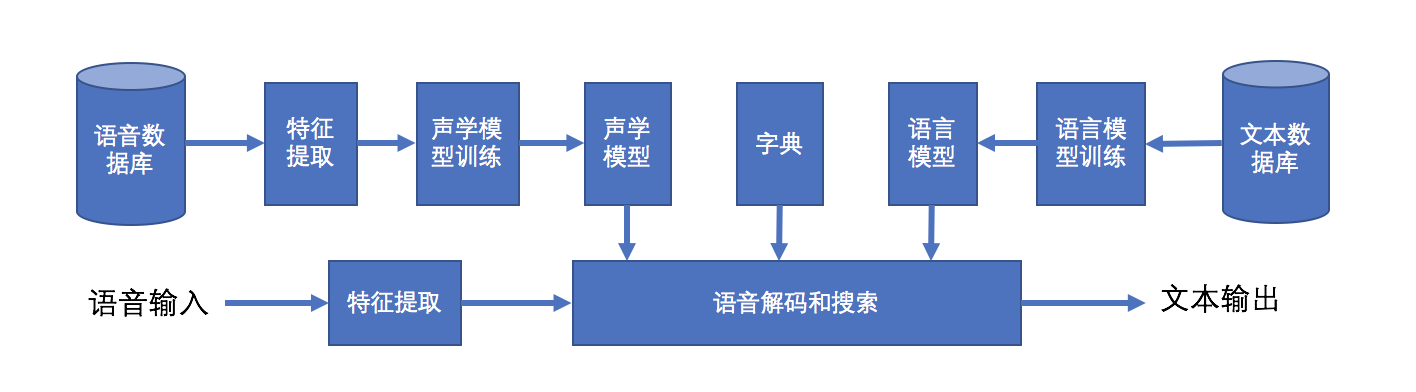
\includegraphics[width=0.9\textwidth]{img/chapter_lm/asr-pipeline2.png}
		\caption{语音音识别基本流程}
		\label{pic:asr}
	\end{center}
\end{figure}

自动语音识别(Automatic Speech Recognition,ASR)是一种将人的语音转换为文本的技术,它是目前很多互联网产品如语音助手,语音搜索引擎等中必不可少的一部分。
图~\ref{pic:asr}给出了常见的语音识别系统的基本工作流程。其中基本可以分为以下几个模块:
\begin{itemize}
    \item 数据预处理: 典型的预处理包含静音处理(Voice Activity Detection,VAD)等,用于去除其中的静音片段。
	\item 特征提取:将声音转换成包含声音信息的多维向量,常见的有MFCC等。
	\item 声学模型:主要是通过语音数据训练得到,其输出是音素等信息。
	\item 词典:字/词和音素之间的对应关系。
	\item 语言模型:也就是上文提到的语言模型部分,主要用于评估字或者词序列的概率。
\end{itemize}

\noindent 语音系统首先将语音信号做特征提取工作,转化成诸如MFCC等特征来表示,然后使用语言模型和声学模型来解码,解码过程会产生很多候选(Candidates),最终最优的候选会被输出成为最终的结果。语言模型是其中很重要的一部分,它用于从根据语言统计规律评估声学模型给出的句子序列候选的概率,决定了最终输出的结果。 
\section{主题模型}

\subsection{基本概念}
主题模型 (Topic Models) 是近些年来非常重要的一项技术,它被广泛应用于工业和学术界。在主题模型中,我们一般用$d$来表示要分析的文档,例如一篇文章或者一个网页等,而一个文档$d$通常由一系列词$(w_1, w_2, ..., w_n)$组成, 其中$w_n$ 是文档中的第$n$个词。多份文档共同构成了我们要分析的语料集,我们用$\mathcal{D}$来表示,$\mathcal{D}=(d_1, d_2, ..., d_m)$组成,其中$d_m$ 是语料库中的第$m$个文档。主题一般用$z$来表示,它由一些词组成,同时也有该词在这个主题下的概率。
主题模型泛指由一类可以从语料库中抽取主题并利用这些主题表示文档的模型,常见的主题模型有PLSA,LDA,以及各种LDA的变种,例如SentenceLDA等。在熟悉了这些基本概念之后,我们通过一种常见的主题模型Latent Diriclet Allocation (LDA)来认识主题模型。




\subsection{常见的主题模型:LDA}

2003年Blei等人在《Latent Dirichlet Allocation》~\cite{blei2003latent} 一文中提出了LDA模型。
如图\ref{pic:lda}所示,其中空心节点表示隐藏变量,实心变量表示客观测变量,整个模型具有K个主题,M个文档和N个词。
LDA将文档的主题分布$P(z|d)$看做随机变量$\theta$,并且假设$\theta$从一个狄利克雷先验中产生。
同时,由于训练数据之外的文档对应的主题分布$\theta$可以从上述狄利克雷分布中产生,训练数据之外的文档的$\theta$可以更自然地进行计算。

\begin{figure}[htb]
	\begin{center}
		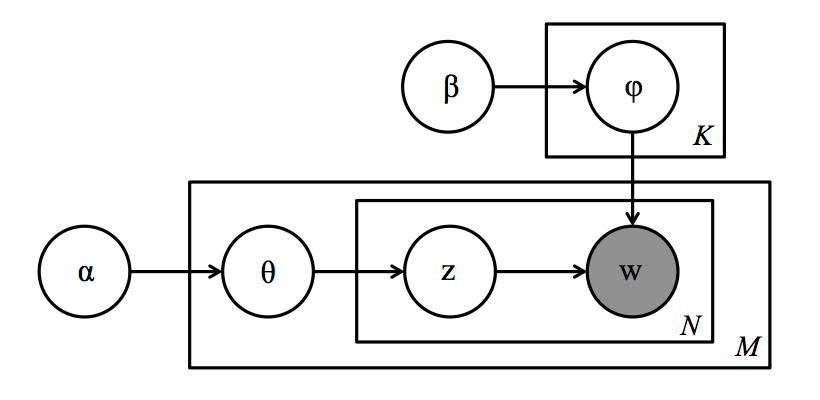
\includegraphics[width=0.8\textwidth]{img/chapter_lm/lda.png}
		\caption{LDA图模型}
		\label{pic:lda}
	\end{center}
\end{figure}

\subsection{主题模型在语音识别中的应用: 语言模型适配}

\begin{figure}[htb]
	\begin{center}
		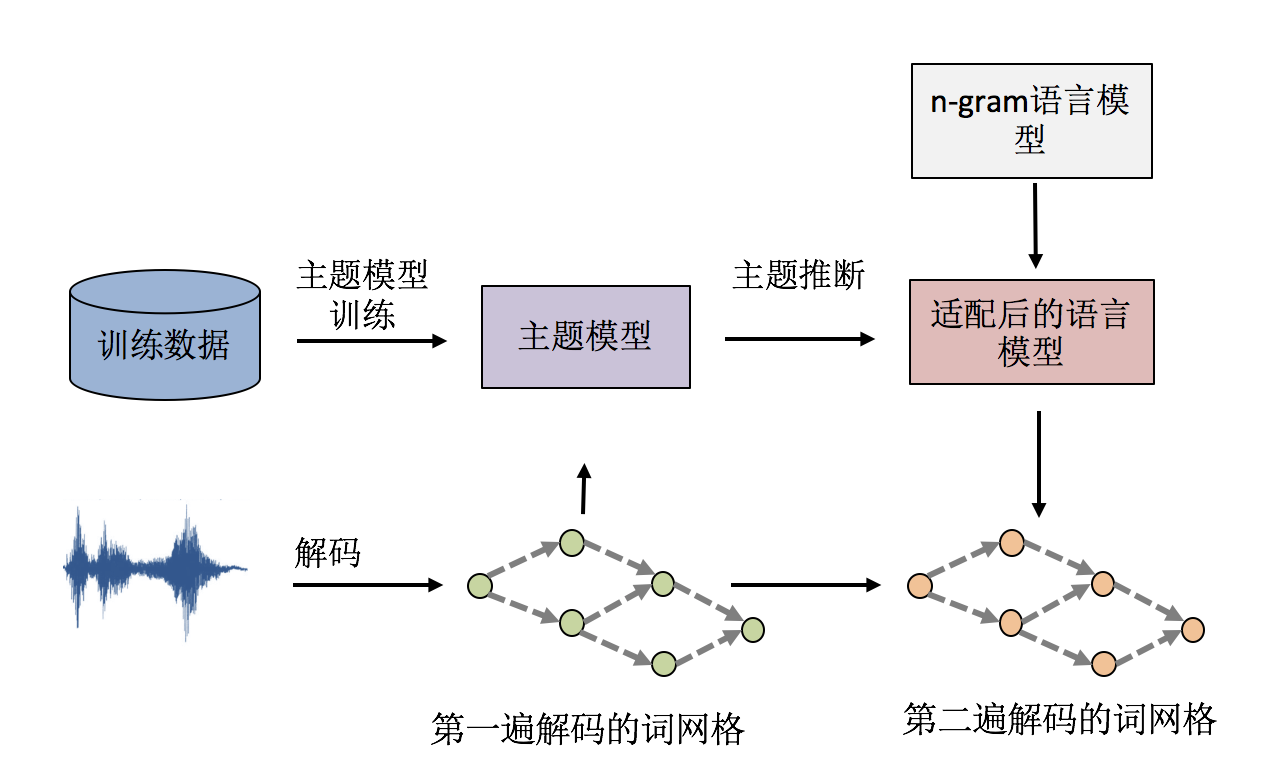
\includegraphics[width=0.8\textwidth]{img/chapter_lm/lma2.png}
		\caption{语言模型适配}
		\label{pic:lma}
	\end{center}
\end{figure}

语音识别系统中一个常见的问题就是,我们训练语言模型的语料和它实际线上应用的语料之间存在不一致,这种情况下,除了重新训练模型,有一种代价更小的方法就是语言模型适配(Language Model Adaptation)。
语言模型适配指的是用实际应用的语料相关的信息,对语言模型做适配。图~\ref{pic:lma}给出了其常见的工作流程,采用预先训练好的主题模型,我们对语音识别系统第一遍识别出来的词网格
(Word Lattice)做主题推断,可以发现其语义级别的内容,同时它也可以作为一个unigram的语言模型$P_{LDA}(w|\theta_d)=\sum_{k \in K} \varphi_{kw} \theta_{dk}$,对之前的n-gram语言模型就行适配:
\begin{equation}
\begin{aligned}
P_{d}(w|C) = \lambda P_{LDA}(w|\theta_d) + (1-\lambda) P_{n-gram \ LM}(w|C)
\end{aligned}
\label{eq:hb_model}
\end{equation}
其中$C$代表当前词$w$的上下文,$\lambda$是一个权重参数,$P_{n-gram\ LM}(w|C)$是基础的ngram语言模型给出来的评估分数。这个新适配过的语言模型,可以用于语音识别系统,重新解码出新的词网格以及最终的结果。


\chapter{词法,语法与语义分析}
\label{basic} % Always give a unique label
% use \chaptermark{}
% to alter or adjust the chapter heading in the running head

\section{词法分析}
\subsection{问题定义}
词法分析是自然语言处理的第一步,要做NLP深层次分析,比如句法分析、语义分析,甚至NLP复杂应用的先决条件,就是首先进行词法分析。词法分析的核心是,将自然语言解析为一个个词的序列,并判断每个词的词性、专名信息,为后续分析做好准备。总的来说,在中文这种孤立语中,词法分析主要由分词、词性标注、命名实体识别3个子任务组成。在英语、阿拉伯语等屈折语中,词法分析一般还包括词根还原(Word Stemming)任务。忽略词根还原,词法分析可以归纳为3个具体的子任务:

\begin{itemize}
\item 自动分词(Word Segmentation):是将连续的自然语言文本,切分成具有语义合理性和完整性的词汇序列的过程。
\item 词性标注(Part-of-Speech Tagging):是指为自然语言文本中的每个词汇赋予一个词性的过程。
\item 命名实体识别(Named Entity Recognition,也称专名识别):是指识别自然语言文本中具有特定意义的实体,主要包括人名、地名、机构名、时间日期等。
\end{itemize}

\begin{figure}[h!]
\centering
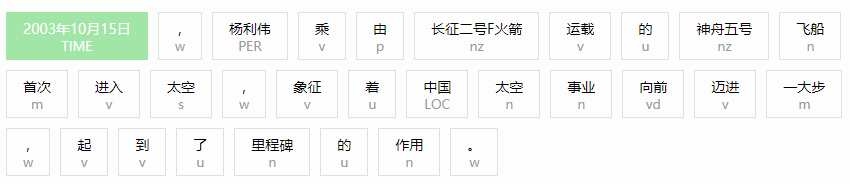
\includegraphics[scale=0.5]{img/chapter_nlp/lexical_example.png}
\caption{词法分析示例}
\label{fig:lexical_example}
\end{figure}

如图\ref{fig:lexical_example}所示,将输入句子切分成一个个词汇,然后给每个词汇标记出名词、动词、介词等词性;并且识别出“2003年10月15日”是一个时间专名,识别“杨利伟”是一个人名专名等。

因为词法分析的自动分词、词性标注、专名识别本质上是类似的,所以它们的发展历史方也是类似的。总结起来,都大致经历词典匹配、机器学习、深度学习这3个发展阶段。

\subsection{实现方案}

\subsubsection{词典匹配}
\noindent
基于词典匹配的实现步骤:

\begin{enumerate}
\item 词典构建:根据具体子任务的语言学知识构建词典。如果是自动分词,则收录常见的词条短语;如果是词性标注、专名识别,则收录当前常见词条对应的名词、动词、介词、专名类型等属性,并且保留相应词性、专名属性的概率。词典构建,通常需要人工收集、整理、离线更新,维护成本较高。
\item 词典匹配:扫描输入的所有子序列,如果当前子序列能够匹配词典中某个词条,则当前子序列属一个可能的候选。如果是分词,则当前子序列就可能为一个分词的词汇;如果是词性标注、专名识别,则当前子序列以相应的概率取词典中的词条属性。
\item 歧义消解:由于候选子序列之间存在歧义,所以基于词典匹配之上,需要加入一些启发式规则以解决歧义问题。常用规则主要包含最大前向匹配(Forward Maximum Matching,FMM)、最大后向匹配(Backward Maximum Matching,BMM)、最少切分、双向最大匹配、长片段优先等策略\cite{wong1996chinese}\cite{weichun2013research}。
\end{enumerate}

中文分词如图\ref{fig:word_segmentation_example}所示。输入序列进行词典匹配之后,得到对应的DAG图,图中每条边都是词典词条,边的权重都为1,图中每一种首尾贯通的连接都是一种歧义切分的候选结果。比如由此只要求解DAG图的最优路径,则可以得到输入序列对应的分词结果。

\begin{figure}[h!]
\centering
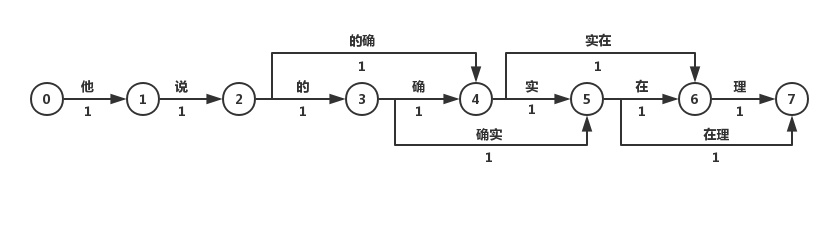
\includegraphics[scale=0.4]{img/chapter_nlp/word_segmentation_example.jpg}
\caption{中文分词示例}
\label{fig:word_segmentation_example}
\end{figure}

很长一段时间内研究者都在对基于词典匹配方法进行优化,比如最大长度设定、字符串存储和查找方式以及对于词表的组织结构,比如采用TRIE索引树\cite{yang2012enhanced}、哈希索引\cite{li2003new}等、AC自动机\cite{ngword}等结构方便快速查找。

基于词典匹配的优缺点:
\begin{itemize}
\item 优点:实现简单、运行速度快
\item 缺点:面临词典收录更新困难、未登录词难处理;同时由于消除歧义策略过于简单,通常效果不甚理想。
\end{itemize}

\subsubsection{机器学习}
\noindent
基于机器学习的实现步骤:

\begin{enumerate}
\item 转换为序列标注任务:词法分析3个子任务,都通过定义标注空间标签集,将具体任务转换为标准序列标注任务。以中文分词为例:转换方法为,标注每个字在其所属词中的位置。因为对于任何一个字来说,它可以是一个词的开始(Begin), 一个词的中间(Inside), 一个词的结尾(End),或者本身就是一个单字的词(Singleton),这也就是在分词序列标注中常用的BIES的分类。只需将输入序列的每个字标上BIES标签中的一个,就可以转换得到对应的分词结果。这种标注空间(模型状态空间)的划分在词性标注和专名识别任务上也很常用,也会有一些类似的变种,比如专名识别中常用BIO标签集。
\item 求解序列标注任务:传统序列标注模型主要包括隐马尔科夫模型(Hidden Markov Model)\cite{zhang2003chinese}\cite{kupiec1992robust}\cite{yu2006chinese}\cite{morwal2012named}、最大熵马尔科夫模型(Maximum Entropy Markov Model)\cite{mccallum2000maximum}\cite{ratnaparkhi1996maximum}\cite{borthwick1999maximum}、条件随机场(Conditional Random Field)\cite{zhao2006improved}\cite{constant2011mwu}\cite{ekbal2008named}、结构化感知机(Structural Perception Machine)\cite{zhang2007chinese}\cite{zhang2008joint}等浅层模型。这些浅层模型的区别主要在于如何对待输入字序列和标签序列之间的概率,训练目标是最大联合概率似然、最大条件概率似然,还是最小化风险等。
\end{enumerate}

总结来说:传统序列标注模型中,CRF是集大成者。相比于HMM,CRF去除了输出独立性要求,对于整个序列内部的信息和外部观测信息都可以有效利用,可以更加有效建模上下文。相比于MEMM,CRF通过全局归一化(global normalization),避免了MEMM locally normalized导致的label bias缺陷。

以自动分词任务为例,则其序列标注任务定义为:
定义标签集为$L=\{B, I, E, S\}$,给定输入文本序列$X=\{x_{1}, x_{2}, ..., x_{n}\}$,目标是求解最优标注序列$Y^{*}=\{y^{*}_{1}, y^{*}_{2}, ..., y^{*}_{n}\}$:

\[y^{*}=\mathop{\arg\max}\limits_{Y \in L^{n}} p(\bm{Y}|\bm{X})\]

预测时,使用维特比算法求解最优标注序列$Y^{*}$;训练时,使用最大化条件似然来训练模型,其中,$f_{i}$为人工定义的特征函数:

\[P_{w}(Y|X)=\frac{1}{Z_{w}(x)}\exp(\sum_{i} w_{i} f_{i}(y_{i}, y_{i-1}, x))\]

\[Z_{w}(x)=\sum\limits_{y \in Y}\exp(\sum_{i} w_{i} f_{i}(y_{i}, y_{i-1}, x))\]

\noindent
基于机器学习的优缺点:
\begin{itemize}
\item 优点:通过人工设计的特征工程,充分地挖掘了序列的上下文信息。模型的歧义消解胜过词典匹配的方法;同时具有很强的泛化能力,能够很好地处理未登录词问题。
\item 缺点:特征工程不经需要耗费大量人力,而且需要大量语言学知识,设计和寻找有效特征存在较高门槛;另外,这些浅层模型,通常使用离散的binary特征,无法表达复杂先验,比如没法利用词向量。
\end{itemize}

\subsubsection{深度学习}
随着大数据、神经网络、深度学习的快速发展,很多研究提出利用前馈神经网络来解决词法分析\cite{collobert2011natural}\cite{zheng2013deep}任务。总的来说,与前面基于机器学习的方法类似,也是把词法分析任务作为序列标注问题进行求解,只是把人工设计特征函数,改成了使用多层前馈神经网络进行自动特征抽取。

\begin{figure}[h!]
\centering
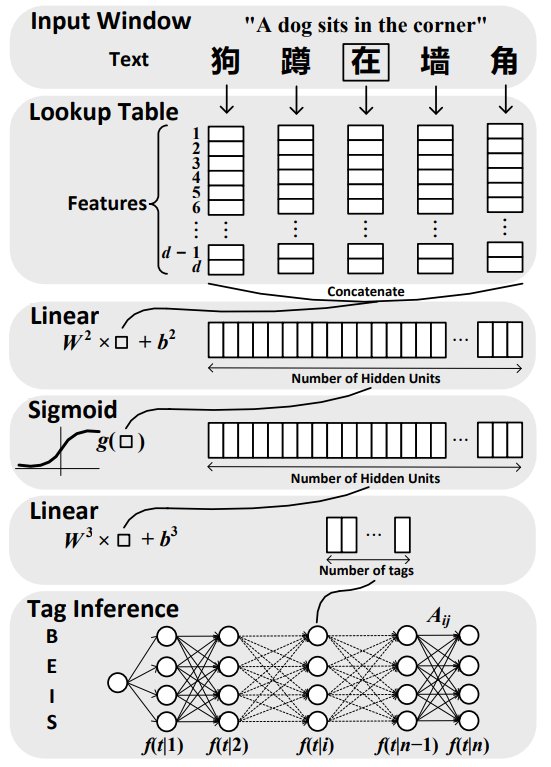
\includegraphics[scale=0.5]{img/chapter_nlp/dl_segmentation_example.png}
\caption{深度学习分词示例}
\label{fig:dl_segmentation_example}
\end{figure}

如图\ref{fig:dl_segmentation_example}所示,网络的第一层输入句子中每个字的字向量,第二层将一个固定长度的字向量进行拼接,然后输入到标准前馈神经网络结构中,神经网络输出在标注集合上的lattice,最后利用维特比算法进行解码,就可以得到最优标注序列。

后续有很多研究,深度学习框架基础上,对前馈神经网络进行改进,进一步探索了卷积神经网络\cite{wu2019neural}、循环神经网络\cite{chen2015long}、递归神经网络\cite{chen2015gated}等复杂结构对词法分析任务的影响。

另外,传统的词法分析通常会把分词、词性标注、命名实体识别当成pipeline形式的进行处理,这样带来的一个问题就是错误传播。比如,分词的错误将会导致后续词性标注、专名识别、句法分析、语义分析出现错误。所以在学术界也有很多联合建模\cite{zhang2008joint}\cite{hatori2012incremental}\cite{shao2017character}方面的工作。联合建模的一大好处是词法分析与其他任务可以共享有用的信息,词法分析的时候也会考虑到其他任务的要求,其他任务也会考虑各种词法分析的可能性,通常可以再全局上取得最优解。但是随之而来问题是搜索的复杂度往往会显著提高:需要更有效的搜索剪枝机制在控制复杂度的同时,不对搜索的结果产生显著影响。

值得一提的是,2018年Peters等证明在利用预训练语言模型\cite{conneau2017supervised}\cite{mccann2017learned}\cite{subramanian2018learning},各种NLP任务都能获得大幅度提升。将语言模型嵌入作为特征,使用目标任务数对语言模型对进行微调\cite{ramachandran2016unsupervised}\cite{howard2018universal},通常就能达到或超过传统结果。由于语言模型只需要无标记的数据便可以进行学习,因此对于标记数据稀缺的低资源场景,预训练语言模型尤其有用。

总结起来,基于深度学习方法的优点是通过深度神经网络自动学习多层特征抽象,避免了复杂的特征工程;模型的歧义消解、泛化能力通常都很好。只是,深度学习模型需要训练充分,通常对数据量、计算量都有较高的要求。

\subsection{应用案例}
通常NLP中深层次的语法语义分析通常都是以词作为基本单位,所以词法分析都是这些深层次分析的基础和先决条件。词法分析作为自然语言处理的第一步,是下游所有分析任务的基础。这些下游应用小句法分析、语义分析,大到对话系统、文本分类、自动摘要、机器翻译\cite{chang2008optimizing}、信息检索、搜索引擎、语音合成等等。几乎只要有利用到自然语言处理技术的地方,词法分析都是不可或缺的基础技术。

比如在搜索引擎中,用户输入一个表述需求信息的查询字段,系统回复一个包含所需要信息的文档列表。其核心技术在于索引构建和相关性计算。

索引构建:首先需要对互联网海量文档进行,分词、词性标注、专名识别;利用词法分析的结果,以词为粒度,为所有文档建立倒排索引。

相关性计算:首先需要对用于查询字段进行词法分析,找出表达用户需求的核心词汇;然后以这些核心词汇为key,去拉取相应的倒排索引,获取初步筛选后的文档;接着,为了要提高返回结果的相关性,需要计算用户查询和初筛文档之间的相似度,取相似度较好的文档返回。其中计算用户查询和文档之间的相似度,通常利用BM25、语义计算等技术,而它们也都是以词为单位进行的,由此看出词法分析在搜索引擎中的重要性、基础性。

在比如在文本分类和情感分类中,在预定义分类体系下,输入给定文本,抽取文本特征,将给定文本于一个或多个类别相关联的过程。其中,抽取文本特征的时候,通常也都是先进行词法分析,先获得给定文本的词汇、词性、专名等信息,然后以词汇为单位,以词汇的词向量、词性专名等信息为特征,利用机器学习、深度学习的分类模型进行预测。


\section{语法分析}
\subsection{问题定义}
短语结构语法(Constituency Structure Grammar)和依存关系语法(Dependency Grammar)是现在常见的两种语法关系。短语结构语法又叫上下文无关文法 (Context-Free Grammars,CFGs),它从一个特殊的初始符号出发,不断的应用一些产生式规则,从而生成出一个字串的集合(如句子)。产生式规则指定了某些符号组合如何被另外一些符号组合替换。
它呈现一个树分类关系,句法根据一定的规则进行转换分析。每一个词的转换都是需要按照设定的树值规则进行目的性的转换。

依存语法(从属关系语法) 是由法国的语言家Lucien Tesnière提出的\cite{tesniere1959elements},
它将句子各个词语之前的搭配关系描述成预先定义好的依存关系。它基于一个基本假设:句法结构本质上包含词和词之间的依存(修饰)关系。一个依存关系连接两个词,分别是核心词(head)和依存词(dependent)。依存关系可以细分为不同的类型,表示两个词之间的具体句法关系。比如主语依赖于谓语(SBV),宾语也依赖于谓语(VOB)以及定语依赖于名词性短语(ATT)等。依存句法认为“谓语”中的动词是一个句子的中心,其他成分与动词直接或间接地产生联系。

除了以上介绍的两种句法体系外,国内外都开展了对句法分析的研究。不论是国外的链语法(Link Grammar) 、组合范畴语法(Combinatory categorial grammar,CCG)等,还是国内黄曾阳教授提出的HNC理论(Hierarchical Network of Concept)\cite{黄曾阳:12}都是目前行业内常用的语法,只是由于设定区域的不同,所以使用有一定的局限性。

短语结构分析的语法集是由固定的语法集组成,较为固定和呆板,依存语法则更加的自由。另外依存语法树标注简单且parser准确率更高,再加之通用依存数据集(Universal Dependencies Treebanks)的发展,依存语法分析受到专家学者普遍的青睐,得到越来越多的应用。这里也将着重介绍依存语法分析。

\begin{figure}[h]
\centering
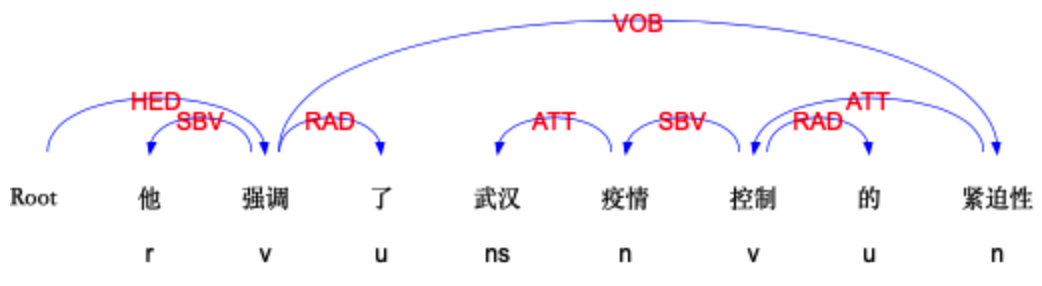
\includegraphics[scale=0.3]{img/chapter_nlp/parser_example.png}
\caption{LTP依存句法分析样例}
\label{fig:parserexample}
\end{figure}
例如,从上述例子中我们可以看到,句子的核心谓词为“强调”,主语(SBV)是“他”,强调的宾语(VOB)是“紧迫性”,“紧迫性”的修饰语(ATT)是“武汉疫情控制”。


\subsection{实现方案}
依存句法分析方法主要可以分为两种,一种是基于图的方法(Graph Based),一种是基于转移(Transition Based)的方法。基于图的方法先建立句子中所有词语的全连接图,然后求图中的最大生成树。 两种方法中更主流的算法是基于转换的依存句法分析,基于转移的方法将依存树的构成过程建模为一个动作序列,将依存分析问题转化为寻找最优动作序列的问题。通过 SHIFT, LEFT\_ARC, RIGHT\_ARC三个动作来将序列转换为树结构。一次分析任务$C = (s, b, A)$由一个Stack栈 $s$,一个buffer缓冲区 $b$,一系列依存弧列表$A$构成。初始化栈$s$里面只包含一个$root$元素即根元素,$s_1$代表栈顶元素,$s_2$表示栈顶第二个元素。缓冲区$b$是一个队列,里面包含了要解析的一句话的序列,$A$为空。一条依存弧有两个信息:动作类型+依存关系名称$l$。$l$视依存句法语料库中使用了哪些依存关系label而定。动作SHIFT将缓冲区$b$ 中最上面的一个词$b_1$移到stack中,即不建立依存关系,只转移句法分析的焦点,即新的左焦点词是原来的右焦点词,依此类推。LEFT\_ARC,即添加栈顶两个词 $s_1$,$s_2$之间的依存边,方向为$s_1 \rightarrow s_2$,并且将$s_2$ 从栈$s$中删除。RIGHT\_ARC,即添加栈顶两个词 $s_1$,$s_2$之间的依存边,方向为$s_2 \rightarrow s_1$,并且将$s_1$ 从栈$s$中删除。

比如图\ref{fig:parserexample}中,首先模型判断执行SHIFT动作将“他”移到栈$s$上,然后再执行SHIFT动作将“强调”移到 栈$s$上,接着模型判断这两个词之间有依赖关系,且方向为为“$\text{强调} \rightarrow \text{他}$”,执行RIGHT\_ARC动作在$A$中添加一条依存弧,且将“他”从栈$s$中删除。接着模型判定执行SHIFT动作将“了”移到盏$s$上,然后模型判断执行LEFT\_ARC操作,即添加“强调”和“了”之间的依存弧“$\text{强调} \rightarrow \text{了}$”到$A$中且将“了”移出栈$s$。如此往复,直到最后当缓冲区 $b$为空和栈$s$只有$root$时结束。训练模型的主要目标即寻找一个分类器,当给定一个Configuration (当前的stack,buffer,依存弧列表)时预测下一步转移的操作类别。

基于转移的解析过程是线性的,动作步骤随句子长度线性增长,而基于图的方法需要在全图上做搜索,所以时间复杂度上基于转移的方法会有优势。但是基于转移的方法在解析的每一步都只是利用局部信息,会导致错误传播,性能比基于图的略差。

近几年,分别出现了针对这两种不同方法的神经网络模型。比如基于图的\cite{dozat2016deep, ji2019graph, ma2017neural},直接用神经网络来预测每两个词之间存在依存关系的概率,得到一个全连接图,图上每个边代表了节点 $a$ 指向节点 $b$ 的概率, 然后使用MST等方法来来将图转换为一棵树。概率的计算可以简单的使用节点$a$和节点$b$的embedding向量做向量运算,也可以使用复杂的多层GNN网络迭代更新。 基于转移的如 \cite{fernandez2019left, kiperwasser2016simple, ma2018stack},通过两个LSTM 来分别建模stack状态、buffer状态,使用第三个LSTM网络或者Pointer网络来建模动作序列。 
\begin{figure}[h]
\centering
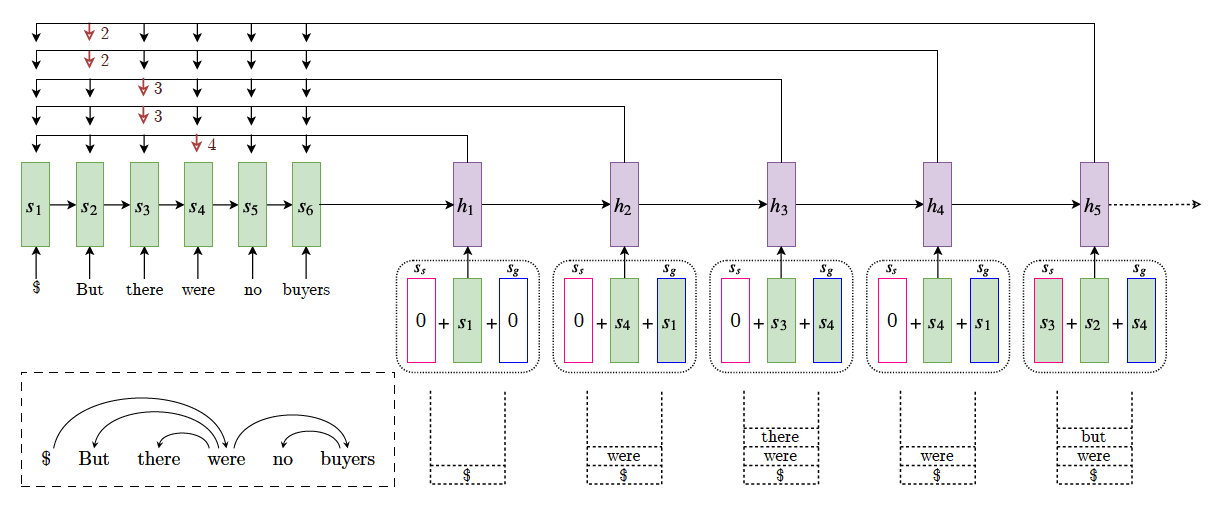
\includegraphics[scale=0.3]{img/chapter_nlp/parser_nn.png}
\label{fig:parser_nn}
\end{figure}


\subsection{应用案例}
依存语法分析在信息检索,评价抽取和情感分析等NLP任务上都有很多应用。比如“谢霆锋的儿子是谁”和
“谢霆锋是谁的儿子” 两句话如果不使用依存语法分析,很有可能就返回了一样的结果。依存句法分析能够更直接地通过语法结构的规则约束筛选出可能正确结果,提升相应任务的准确性。又比如“深圳大学非常漂亮,学生都很聪明”,这里 “漂亮” 形容的是 “深圳大学”, “聪明”形容的是“学生”,通过依存句法分析,就可以抽取出对应的搭配。再比如“我家音响声音很大”和“我家洗衣机声音很大”,两者在情感上前者是正评价,后者是负评价,需要使用依存句法分析来识别“声音很大”的修饰对象。

常用的中文依存句法分析的工具有复旦大学fnlp\footnote{\url{https://github.com/FudanNLP/fnlp}},斯坦福大学 Stanford CoreNLP\footnote{\url{https://stanfordnlp.github.io/CoreNLP/}}, Hanlp\footnote{\url{https://github.com/hankcs/HanLP}}和哈工大 LTP\footnote{\url{https://github.com/HIT-SCIR/ltp}}。





\section{语义分析}
在自然语言处理领域,语义分析涉及在某种程度上理解单词、短语、句子或文档的意义。传统狭义语义分析主要包括语义消歧(word sense disambiguation)\cite{ yarowsky1995unsupervised}和语义角色标注(semantic role labeling)\cite{ carreras2005introduction, bjorkelund2009multilingual}。语义消歧指在给定文本上下文中确定多义词语的含义,例如,“他买了一台新苹果,用来修图更方便了”中,苹果一次指代苹果电脑,而非水果。语义角色标注是给词语和短语标注其在上下文文本中的含义的过程,典型标注标签包括主体、意图、结果等,如图\ref{fig:semantic_role_label}。语义角色标注是面向任务型对话系统中核心组件自然语言解析模块的基础技术之一。

\begin{figure}[h]
\centering
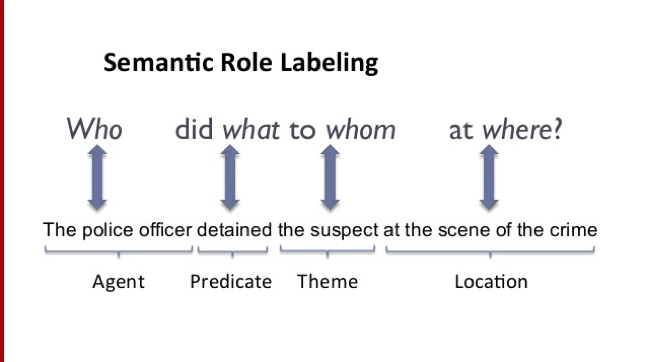
\includegraphics[scale=1]{img/chapter_nlp/guang_analysis_1.png}
	\caption{语义角色标注示例}
\label{fig:semantic_role_label}
\end{figure}

随着深度神经网络在自然语言处理领域的应用和研究,基于神经网络的语义分析得到了越来越多的应用和发展,并成为了驱动神经机器翻译\cite{ bahdanau2014neural, luong2015effective}、阅读理解\cite{ hermann2015teaching}、对话系统\cite{ serban2016building, chen2017survey}的最基础和核心的技术。基于神经网络的语义分析广义上可分为语义表示和语义匹配。其中语义表示任务将词语和短语镶嵌到高维向量空间中,称作词向量,作为CNN\cite{ lecun1995convolutional}、RNN\cite{ hochreiter1997long}和Transformer\cite{ vaswani2017attention}等模型的底层输入,根据任务需要,可以灵活的实现文本分类\cite{ joulin2016bag, zhang2015character}、机器翻译、阅读理解、对话系统、文本摘要\cite{ tan2017abstractive, yao2017recent}等自然语言处理任务,逐步替代或部分替代了传统以ngram one-hot向量作为底层表示的方法。语义匹配任务更多关注句子和篇章层级的语义的相似性,例如,寻找给定语料库中与查询语句语义层面最相似的句子。语义匹配任务在信息抽取、对话系统、问答系统都有广泛的应用。

\subsection{语义表示}
语义表示中词向量的概念可以追溯到Bengio的著作\cite{ bengio2003neural}。作者在文中提出了一种基于神经网络的语言模型,创新的提出将每一个词表示成一个高维的向量,而后使用神经网络计算给定上文词语后,下一个词出现的概率分布,最大化训练语料出现的概率。训练语料是单词序列$w_1, \cdots, w_t, w_t \in V$,其中$V$是全体单词的集合。语言模型的目标是找到一个模型$f(w_t, \cdots, w_{t-n+1}) = P(w_t|w_1 ^ {t-1})$,即在给定前$t-1$个词的情况下,对第$t$个词的概率分布建模。Bengio提出把词表示成实数向量,$C(i) \in \mathbb{R}^m$,即每一个词对应一个维度为$m$的实数向量,映射$C$可以用一个$|V| \times m$的实数矩阵表示。在第二步中,作者提出使用神经网络$g$来建模给定前缀序列下一个词的概率。模型结构如图~\ref{fig:neural_language_model}。
其中,将词表示成高维实数向量的方法是词向量以及一系列神经网络在自然语言处理应用的开端。通常,我们会设计一个仅与文本结构或上下文相关的(无监督)任务作为目标,拟合训练数据,得到词向量表示。在Bengio之后,Word2Vec\cite{ mikolov2013distributed}, Glove\cite{ pennington2014glove}, ELMo\cite{ peters2018deep}等一系列词向量方法出现并逐渐成为自然语言处理的标准工具。
语义表示不仅限于词的层面,广义的语义表示在现代基于神经网络的自然语言处理中应用广泛。例如,神经机器翻译通常采用编码器译码器(Encoder-Decoder)\cite{ sutskever2014sequence}结构,其中编码器的输出可以看做是翻译模型对输入文本的语义表示,译码器基于该表示,生成目标语言的文本。再如,闲聊型对话系统中,需要针对聊天的上文给出合适的回答。闲聊对话系统可以分为生成式对话系统(Generation-based)\cite{ shang2015neural}和选择式对话系统(Selection-based)\cite{ chen2017survey}。选择式对话系统依赖语义匹配方法。典型的生成式闲聊对话系统也采用编码器译码器结构,其中编码器的输出是对聊天上文的总结性表示,可以认为是广义上的聊天上文的语义表示,用于在译码器中生成合适的回答语句。此外,随着自然语言处理预训练模型的发展,Bert\cite{devlin2018bert},GPT-2\cite{ radford2019language},MASS\cite{ song2019mass}等预训练模型(Pretrained models)在阅读理解等任务上大放异彩。这些模型可以看做是多个联合任务共享底层语义表示的学习,通常使用与文本结构相关的目标作为训练目标,设计神经网络结构表示文本。在应用时,这些预训练获得的表示仅需在少量标注数据上进行优化,即可获得优秀的子任务模型。通常,编码器和预训练模型采用CNN、RNN、Transformer等结构处理文本序列,在CNN和RNN中通常还会使用注意力(Attention)机制,得到文本片段的语义表示。

\begin{figure}[h!]
\centering
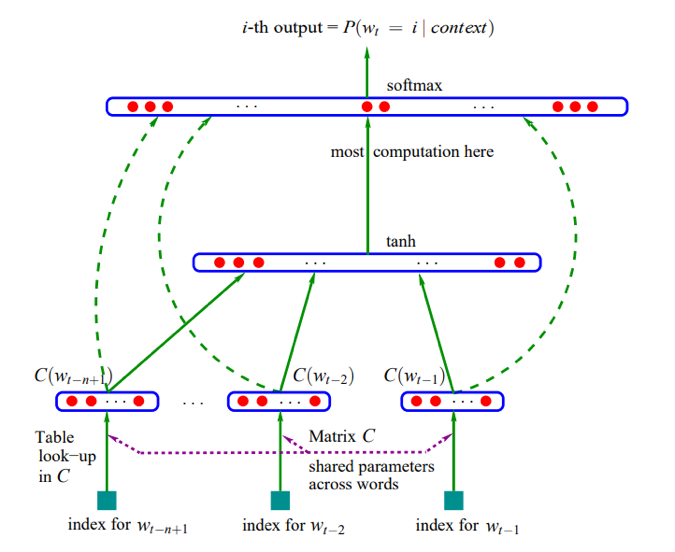
\includegraphics[scale=1]{img/chapter_nlp/guang_represent_1.png}
	\caption{一种使用词向量的神经语言模型结构}
\label{fig:neural_language_model}
\end{figure}

\subsection{语义匹配}
语义匹配任务在语义表示的基础上,对文本片段之间的相似度或相关度给出量化指标,语义越相似的片段匹配分数越高。语义匹配可大致分为基于表示的匹配(representation-based matching)\cite{ feng2015applying}和基于交互的匹配(interaction-based matching)\cite{ zhou2018multi, luspatio}。
基于表示的匹配方法注重对表示层的构建。常见的匹配度计算方式包括cosine函数,和神经网络匹配,如图~\ref{fig:representation_based_matching}。Cosine函数直接计算待匹配对的语义表示向量间的cosine值,通常cosine值越大代表待匹配对的相似度或相关度越高。这种方法不需要额外的训练数据,实现简单并且高效,在工业中广泛应用。神经网络匹配方式使用一个额外的神经网络结构,将待匹配对的语义表示向量作为输入,计算语义匹配分数。这种方法更加灵活,可根据数据定制匹配结构。但需要额外的标注数据进行训练,才能得到可用的匹配模型。

\begin{figure}[h!]
\centering
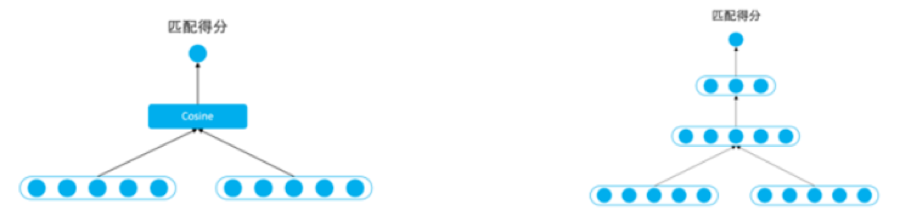
\includegraphics[scale=0.8]{img/chapter_nlp/guang_match_1.png}
	\caption{基于表示的匹配}
\label{fig:representation_based_matching}
\end{figure}

基于交互的匹配方法通常会保留待匹配对的序列信息,不会在表示层将文本转换成唯一的一个整体向量表示,而保留一个向量序列,用于接下来的交互匹配过程。例如将句子表示成一个与句子等长的向量序列。该向量序列可以使用语义表示的方法得到,例如使用RNN对文本序列进行建模。得到待匹配的序列对后,可以对序列中每个位置的向量计算与待匹配序列中向量的相关度。对每一个位置使用相同的方式计算相关度,可以得到一个匹配矩阵(matching matrix)。匹配矩阵包含了更细致的局部文本交互信息,在交互矩阵的寄出上,我们可以构建神经网络结构计算最终匹配得分,去拟合目标得分。图~\ref{fig:interaction_based_matching}展示了一个典型的基于交互的语义匹配方法在选择式对话系统中的结构。其中Representation module对应语义表示部分,matching block对应交互匹配部分。

\begin{figure}[h!]
\centering
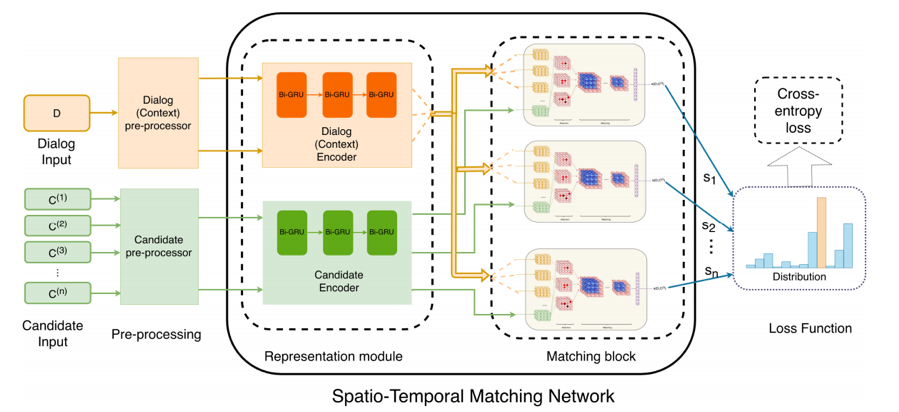
\includegraphics[scale=0.8]{img/chapter_nlp/guang_match_2.png}
	\caption{基于交互的匹配}
\label{fig:interaction_based_matching}
\end{figure}


%%%%%%%%%%%%%%%%%%%%% chapter.tex %%%%%%%%%%%%%%%%%%%%%%%%%%%%%%%%%
%
% sample chapter
%
% Use this file as a template for your own input.
%
%%%%%%%%%%%%%%%%%%%%%%%% Springer-Verlag %%%%%%%%%%%%%%%%%%%%%%%%%%
%\motto{Use the template \emph{chapter.tex} to style the various elements of your chapter content.}
\chapter{对话理解与智能质检}
\label{basic} % Always give a unique label
% use \chaptermark{}
% to alter or adjust the chapter heading in the running head
本节首先给出对话理解任务的定义,然后介绍对话理解的主要方法。接下来以智能质检为例,讲述对话理解是怎么落地和实现的。
\section{对话理解}
\subsection{什么是对话理解}
对话理解是指希望计算机跟人一样,具备自然语言理解的能力,从对话内容中挖掘对话意图,理解对话意图,用户情绪识别等。例如,在客服与用户交互的对话中,用户询问“今天的天气如何”,这里就是一个“询问天气”的意图。在实际对话中,
由于自然语言的多义同义问题,语言的词序问题,我们不能只停留在字面理解层面,更需要语义层面的理解。

这里对话可以包含语音对话和文本对话,如果是语音对话,我们一般可以利用语音自动识别技术将语音转为文本。后续我们要讨论的内容是文本的对话理解。
\subsection{技术路线简介}
一般而言,文本的对话理解从技术角度上可以分为两类:文本匹配和文本分类。

\textbf{文本匹配}~~~文本匹配的目标是得到$f(text_1, text_2)$的语义匹配得分,其中$text_1$和$text_2$是输入的文本,$f$是文本匹配模型。传统文本匹配技术主要按照字面上词汇重合度来进行文本匹配,比如传统信息检索中的向量空间模型VSM、BM25等算法。这种基于词汇重合度的匹配算法存在一定的局限性。例如“出租车”和“的士”语义是一致的,但是字面上却完全不匹配。近年来,随着深度学习技术的发展,我们通过多层神经网络对文本语义进行建模,在语义匹配效果上有了很大的提升。

深度学习的模型主要包含Representation-based Match和Interaction-based Match两种,如下图所示。

\begin{figure}[ht]
\centering
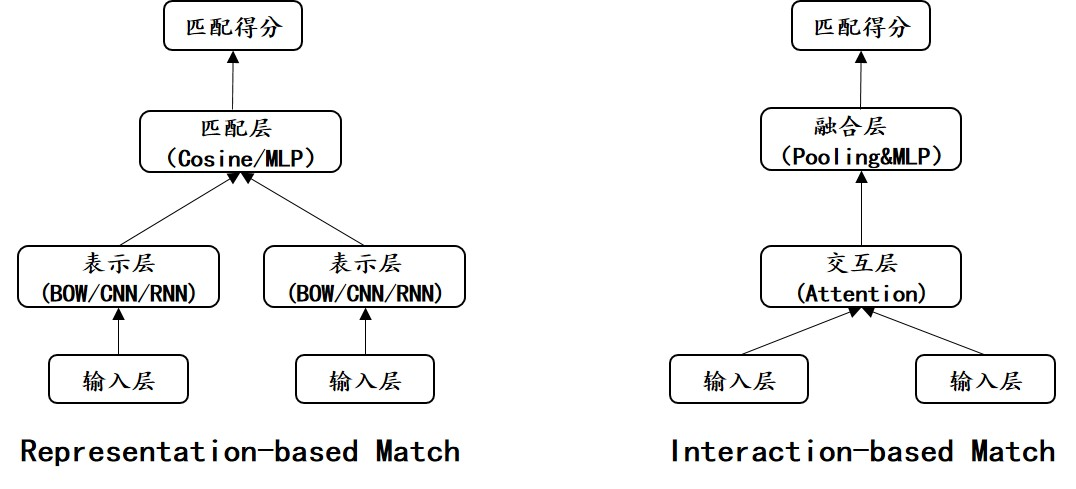
\includegraphics[scale=0.6]{./img/chapter4_b/representation-interaction.jpg}
\caption{Representation-based Match和Interaction-based Match框架图}
\label{fig1}
\end{figure}
输入层一般是将词通过look-up table变成词向量,常见的方法有word2vec, 其后陆续出现了一些文本向量化方法, 如GloVe, FastText, EMLo等,不过word2vec几乎还是最适用的方法之一。词到向量的转化使得词与词之间的语义相似性可以通过向量相似度的方法来度量。为了减少数据稀疏,我们可以加入subword information,即词内的结构信息,中文里面就是字的信息,英文就是字母的信息。

Representation-based Match的核心思想是先将句子转为向量,然后再匹配。怎么获得句子向量呢?最简单的方式有Bag of Words(BOW),句子中词向量求和作为句子向量表示,向量求和可以将不定长的句子转化为定长的向量,但BOW的方式忽略了句子中词序对语义带来的影响。当然,句子向量更高级的获取方式可以使用卷积神经网络(CNN)或者循环神经网络(RNN)来得到。有了句子向量,我们通过匹配层去计算两个句子向量的匹配得分,这里匹配层可以是用余弦距离(Cosine Distance)或者把两个句子向量拼接(concatenation)再经过一个多层感知机(MLP)来实现。经典的方法有Siamese CNN,Siamese LSTM,DSSM,ARC-I等。Representation-based Match的优势是可以离线计算好句子向量的表示,易于建立索引,执行效率高,非常适合文本匹配的粗召回。但其存在的问题是容易丢失语义焦点,词的上下文重要性较难捕捉。

Interaction-based Match则是构造了两个句子之间的语义单元(e.g., term,n-gram,part-of-speech)的交互矩阵,然后再经过一个融合层将细粒度的语义匹配信息合并,较好的把握句子的语义焦点和保留重要的句子间相似信息。主流的方法包含ARC-II,DeepMatch和MatchPyramid等。Interaction-based Match不能离线预处理,需要在线匹配,适合精排序。

\textbf{文本分类}~~~文本分类的目标则是得到${g(text)}$的语义标签,其中$text$是输入的文本,$g$是文本分类模型。文本分类问题需要数据标注其语义标签,在任务型对话中,这个语义标签就是意图。文本分类模型训练好后,我们就可以对新数据进行分类了。具体内容可以参考对话系统的章节。

\section{应用案例:智能质检}
对话理解在智能客服,智能质检有着广泛的应用。下面以智能质检为例,阐述对话理解相关技术是怎么应用的。
\subsection{什么是智能质检}

智能质检使用人工智能算法,分析坐席呼叫场景下人工客服与客户的对话,实现全量质量检查,提高人工客服的服务质量和客户的满意度。
智能质检系统的输入是一通人工客服和客户对话的录音,输出是质检报表,显示该录音在不同质检项的合格情况。质检项的重要性通过质检项的分数来决定。
智能质检无需人工介入,节省质检人力,覆盖率高(100\%),提升质检效率,降低漏检错检率。
\begin{figure}[h]
\centering
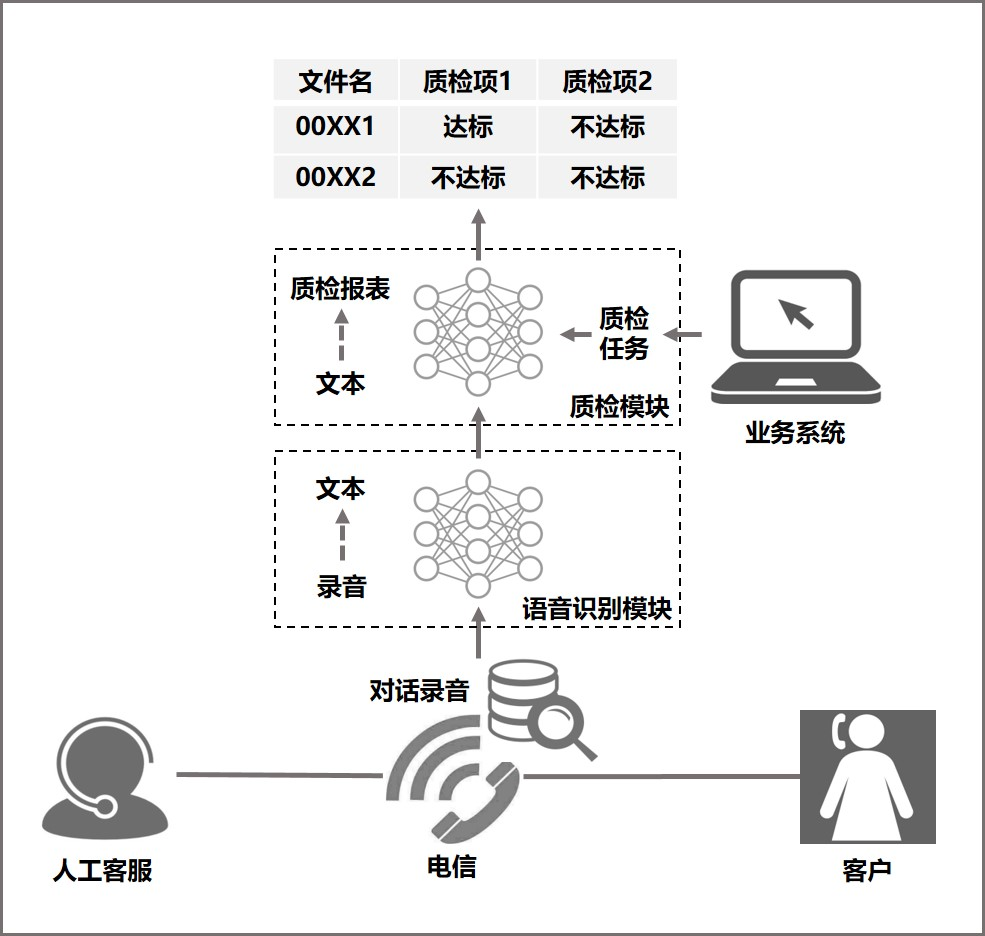
\includegraphics[scale=0.4]{./img/chapter4_b/qic_workflow.jpg}
\caption{智能质检基本流程图}
\label{fig1}
\end{figure}

从智能质检的基本流程图中我们可以发现,对话录音经过语音识别模块之后,我们得到了客户和人工客服之间的对话文本。质检员配置了质检项之后,我们将对话文本输入质检模型,最后得到了质检报表。
\subsection{实现方案与应用状况}
\textbf{实现方案}~~~假设我们定义了质检项要求客服在对话中“核实用户的工作地址”,比如“你的公司地址在哪里”。一种简单的实现方案是通过规则配置“算子+逻辑操作符”或者正则表达式,如果录音文本中满足匹配条件,则命中该质检项。我们可以配置“(公司|工作)\&地址\&(哪|地方)”这样识别出“你的公司地址在哪里”和“您的工作地址在什么地方”这两种说法。这里“公司”就是一个关键词算子,“\&”是一个“与”的逻辑操作符,“|”是一个“或”的逻辑操作符。
这种本质上还是一种基于词汇重合度的匹配算法,适合冷启动,在没有标注数据的情况下就能构建一个简单的质检系统。但它也存在诸多弊端:第一、配置规则需要一定的专业知识,有培训成本;第二、当质检项和表达方式增多时,不同质检项容易出现规则冲突,维护成本高;第三,对于一些比较复杂的质检项,很难通过配置规则进行质检,容易出现漏检和误检的问题。

如果我们有标注数据,就可以使用文本匹配和文本分类的方法。计算$f$(录音文本,质检例句)的语义匹配得分或者$g$(录音文本)的质检项标签。为了减少对数据的依赖和利用大量的无标签数据,一种有效的做法是在BERT(Bidirectional Encoder Representation from Transformers)模型上去fine-tune分类器,BERT用于上层模型的特征提取,作为上层模型的输入,它能够较好的捕捉对话片段的高层语义,兼容少量的漏字情况。我们通过数据驱动的方法让模型越来越聪明,业务方只需要提供标注数据就能进行质检,不需要人工定义规则,模型具有一定的泛化能力。但遇到bad case没有基于规则的方法容易修复,另外需要标注数据积累到一定规模才能发挥模型的优势。

\textbf{应用状况}~~~当前智能质检的应用可以包含离线质检和坐席实时质检。离线质检是指结合语音识别和自然语言处理技术,对海量录音数据进行智能化分析。离线质检可对全量录音质检,质检过程无需人工介入,可以提供内容质检,敏感词识别,语速分析等质检结果。坐席实时质检是指在人工客服和客户对话过程中,提供实时质检能力,辅助人工客服判断客户情绪和实时分析对话过程的信息,及时提醒人工客服从而使客户获得更好的服务。现在智能质检的产品形态包含SaaS云服务和私有化部署。SaaS级产品部署,让中小企业也能够享受智能质检带来的高效与便捷,克服了采购费用高部署周期长的问题。

未来随着多方业务的使用,可以基于联邦学习进行智能质检,在满足数据安全和私隐保护的前提下,通过模型的参数梯度共享,获得了把所有数据放在一起训练的效果,使得不同的业务方合作共赢,建立更准确的数据模型。


%%%%%%%%%%%%%%%%%%%%% chapter.tex %%%%%%%%%%%%%%%%%%%%%%%%%%%%%%%%%
%
% sample chapter
%
% Use this file as a template for your own input.
%
%%%%%%%%%%%%%%%%%%%%%%%% Springer-Verlag %%%%%%%%%%%%%%%%%%%%%%%%%%
%\motto{Use the template \emph{chapter.tex} to style the various elements of your chapter content.}
\chapter{人脸识别}
\label{basic} % Always give a unique label
% use \chaptermark{}
% to alter or adjust the chapter heading in the running head


\section{问题定义}
人脸识别,是指对输入的图像和视频,检测其中存在的人脸,依据人脸的面部特征,完成身份识别的过程,属于生物特征识别技术。整个流程包含人脸检测、人脸对齐、人脸特征提取、人脸匹配几个阶段,如图 \ref{fig:face_recog_flow_chart} 所示。目前人脸识别已经广泛应用于安防、金融、军事等领域。

人脸识别具有以下优点:

自然性:所谓自然性,是指人脸识别技术所利用的生物特征,与人类进行人脸识别时所利用的生物特征是一致的,与之相比,虹膜识别、指纹识别等技术,则不具备自然性。

非接触性:在人脸识别技术中,用户不会与识别设备发生任何接触,对于用户来说体验较好。而指纹识别则需要用户进行按压设备。

使用便捷:用户使用人脸识别技术时非常方便,基本上无需做特殊的配合。

人脸识别也具有一些缺点,比如易受光照条件的影响,易受人脸遮挡物的影响,跨年龄识别难度较高等。但总的来说,人脸识别是目前一种可靠的,实用的,便捷的身份核验技术。

\begin{figure}[ht]
\centering
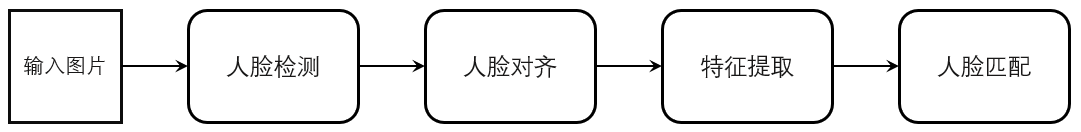
\includegraphics[scale=0.5]{img/chapter_fr/face_recog_flow_chart.png}
\caption{人脸识别流程图}
\label{fig:face_recog_flow_chart}
\end{figure}

\section{实现方案}
\subsection{人脸检测及对齐}
人脸检测是人脸识别的第一步,属于目标检测的子方向。其目的是找出图像中的人脸以及对应的位置。可能还会包含一些人脸的额外信息,比如人脸的关键点,姿态角度等。

典型的人脸检测是基于以下的流程:由于人脸可能出现的图像的任何位置,因此需要通过滑动窗口(sliding windows)来获取可能包含人脸的子图像。获取到的子图像,需要通过一个二分类的分类器,来判断图像中是否包含人脸,如果还需要确定人脸的精确位置,还需要加上一个回归人脸框的操作。同一个人脸可能会检测出多个人脸框,因此需要使用非极大值抑制(Non-Maximum suppression, NMS)来进行合并去重。由于人脸有大有小,为了更好的检测出不同尺度的人脸,还需要输入图像做不同尺度的图像缩放,也叫图像金字塔技术。接下来本文介绍一些具有代表性的人脸检测方法。

Viola-jones\cite{viola2001rapid}是2001年提出的一个人脸检测方法,该方法具有检测效率高,并且能够保持较好的精度的特点,是第一个具有实用意义的人脸检测算法。该方法使用Haar-like小波特征,并通过级联的AdaBoost分类器构造检测器。同时,还是用了积分图来加速Haar-like输入特征的计算。这是一个具有里程碑意义的方法。

MTCNN\cite{zhang2016joint}是2016年提出的一个人脸检测方法,它将人脸分类、人脸框回归以及人脸关键点定位在同一个任务内完成了,是一个多任务(multi-task)的检测方法,这种思路在后续的很多方法里也得到了使用。该方法采用三级网络级联的方法,定义了3个子网络:P-Net,R-Net以及O-Net,P-Net用于快速产生候选框,使用全卷积运算代替了滑动窗口,大大提升效率,R-Net和O-Net用于对候选框进行精细调整。

anchor的思想在Faster-rcnn\cite{ren2015faster}中首先被提出,该方法被广泛应用于两阶段和单阶段的目标检测任务中,在人脸检测中也经常使用到。anchor提出的目的是为了解决目标在图像中可能以不同的形状存在,比如不同的长宽比,所以加入人工的先验信息,预先定义不同比例的anchor来进行候选目标框的获取。Face r-cnn\cite{wang2017face}, Pyramidbox\cite{tang2018pyramidbox}, Retinaface\cite{deng2019retinaface}这些方法,都用到了anchor的思想。另一个在人脸检测中经常使用的思想是特征金字塔网络(feature pyramid network),人脸在图像中,可能以不同尺度的大小出现,为了能够对大人脸和小人脸都有很好的检测效果,一般有两种做法,一种做法是图像金字塔,这种方法需要对输入图像做不同尺度的缩放,缺点是耗时较高;另一种更好的做法则是特征金字塔,其思想是在不同分辨率的特征图(feature map)上检测对应尺度的目标,同时将不同分辨率的特征图与更高层的特征图进行特征融合,保证每一层的特征图都具有足够的表达能力。Pyramidbox,Retinaface都用到了特征金字塔,SSH\cite{najibi2017ssh}虽然没有直接用到特征金字塔,但其也是对网络3个不同尺度的特征图进行分别预测,来解决多尺度的人脸检测问题。

人脸检测检测通常会以检测率、误检率等作为评估指标,同时会关注性能指标。很多算法的效果很好,但性能会很差,做不到实时,也就限制了使用场景。

做完人脸检测后,一般需要进行人脸对齐。通过对人脸进行关键点定位,以及预先定义好的关键点模板,进行仿射变换,通过旋转、平移、缩放等操作,进行人脸对齐,对齐后的人脸能够更好的进行人脸特征提取。目前常见的关键点个数,有5个关键点、68个关键点、90个关键点以及106个关键点等。

\subsection{人脸特征提取}
人脸识别中,最重要的步骤是人脸特征提取,将人脸在高维空间的描述转化为其他空间内的低维描述,使得转化后的特征能够很好地区分不同人之间的差异点。经过特征提取得到人脸的特征表示之后,可以进行特征匹配。如果是对两个特征进行比对,我们一般称为人脸比对或者人脸验证(verification),如果是将一个特征与一组特征进行匹配,我们一般称为人脸检索或者人脸识别(identification),如图 \ref{fig:verification_identification} 所示。匹配的效果直接依赖于特征提取是否准确,因此如何提取好的人脸特征是特别重要的。


\begin{figure}[ht]
\centering
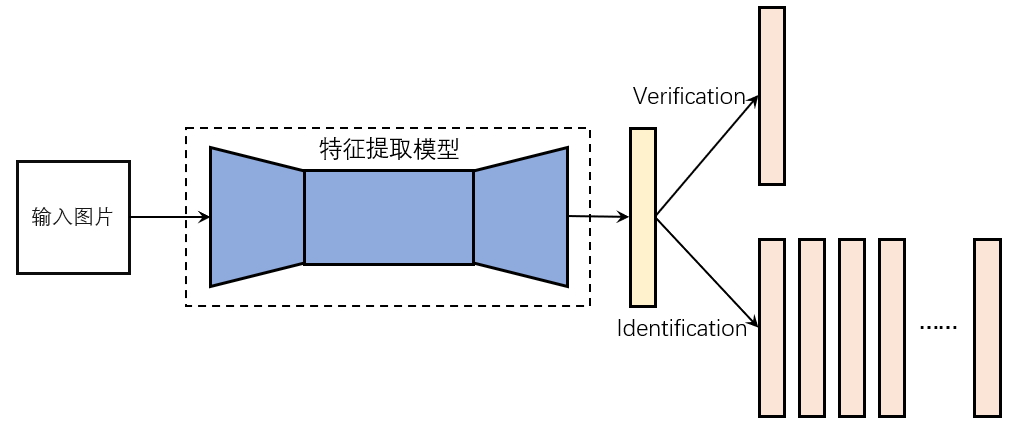
\includegraphics[scale=0.55]{img/chapter_fr/verification_identification.png}
\caption{人脸特征抽取}
\label{fig:verification_identification}
\end{figure}


传统的特征提取算法,通过一些降维方法,得到一系列降维后的特征,用来表示人脸。比如使用PCA进行降维的EigenFace,基于LDA进行降维的FisherFace等,都是早期人脸识别中非常经典的算法。但这些方法存在一些缺点,对光照、表情、姿态敏感,泛化能力不足,因此在实际使用中的准确度不高。

随着深度学习的广泛应用,越来越多具有实用价值的方法被提出,人脸识别的研究得到了极大的发展。基于深度学习的特征提取方法可以分为两大类:
\paragraph{度量学习(metric learning)}
通过一个度量函数,来衡量相同人或者不同人的特征表示之间的距离,从而学习到每个人每个照片的特征表示,基本思路是同一个人的特征表示之间的距离尽可能小,不同人的特征表示的距离尽可能大。
这一个方向的典型方法包含2014年的Contrastive loss\cite{sun2014deep}和2015年google提出的Triplet loss\cite{schroff2015facenet}。

DeepID2是基于Contrastive loss的模型,它在训练的时候,同时训练classification和verification两个信号,其中的verification信号,就是用特征表示之间的Contrastive loss来构造的。Contrastive loss是基于pairwise的思想,模型训练时,需要输入两张图片,如果两个图片是同一个人,则verification的标签为1,如果不是同一个人,则标签为0。

google于2015年提出的Facenet中,则用到了Triplet loss。其思想是以三元组的形式来训练模型,每次输入需要三张图片,其中两张图片是同一个人,以及一张其他人的图片,要求同一个人的照片之间的距离要小于不同人之间的距离,且要超过一个margin。具体公式如下所示:
\[L_{triplet}=\sum_{i=1}^{N}max\{0, \parallel f(x_i^a) - f(x_i^p) \parallel_2^2 - \parallel f(x_i^a) - f(x_i^n) \parallel_2^2 + \alpha \}\]
其中,$f(\cdot)$表示输入图像的特征表示,$x_i^a$表示anchor样本,$x_i^p$表示positive样本,$x_i^n$表示negative样本,$\alpha$表示对应的margin。

\paragraph{基于margin的分类方法(margin based classification)}
第二类思想是基于分类的思想来进行特征提取,根据训练集中的数据,同一个人的照片属于同一类,训练集一共包含多少个id,则总共需要分多少类。由于用的分类的思想,所以自然而然可以使用分类的损失函数。而在此基础上,又提出了一系列的方法,用以最小化类内间距或者最大化类间间距。比较有代表性的方法有Center loss\cite{wen2016discriminative},SphereFace\cite{liu2017sphereface},CosFace\cite{wang2018cosface}以及ArcFace\cite{deng2019arcface}等。

由于是多分类任务,所以最基本的损失函数形式是softmax loss,softmax loss是指概率输出函数为softmax函数,且损失函数为交叉熵(cross entropy)。但是直接用softmax loss训练出来的特征,往往效果不理想,某些类别的类内间距甚至比类间间距大,导致人脸识别的时候出现错误。center loss引入了类内中心,为每个类别提供一个类内中心,最小化训练集中每个样本与其类内中心的距离,从而达到减少类内间距的效果。具体形式如下所示:
\begin{equation*}
\begin{split}
L_{centerloss}&=L_S + \lambda L_C \\
&=-\frac{1}{N}(\sum_{i=1}^{N}log(\frac{e^{W_{y_i}^T f(x_i) + b_{y_i}}}{\sum_{j=1}e^{W_j^T f(x_i) + b_j}}) + \frac{\lambda}{2}\sum_{i=1}^{N}\parallel f(x_i) - c_{y_i}\parallel_2^2) \\
\end{split}
\end{equation*}
其中,$c_{y_i}$表示$x_i$所对应类别的中心,它与$f_(x_i)$的维度一致,该类别中心与参数一样,需要在训练中迭代更新。

基于SphereFace的训练方式,是在此基础上做了改进,对权重进行了归一化,且增加了角度裕量,在cos函数上对角度乘上因子m,加大分类难度。具体形式如下所示:
\[L_{sphereface}=-\frac{1}{N}\sum_{i=1}^{N}log(\frac{e^{{\parallel f(x_i) \parallel_2}cos(m\theta_{y_i,i})}}{e^{{\parallel f(x_i) \parallel_2}cos(m\theta_{y_i,i})} + \sum_{j \ne y_i}e^{{\parallel f(x_i) \parallel_2}cos(\theta_{j,i})}})\]

CosFace和ArcFace更进一步,对特征$f(x_i)$也做了归一化,并分别引入了不同的margin形式,取得了更好的效果,如下所示:
\[L_{cosface}=-\frac{1}{N}\sum_{i=1}^{N}log(\frac{e^{s(cos(\theta_{y_i, i})-m)}}{e^{s(cos(\theta_{y_i, i})-m)} + \sum_{j \ne y_i} e^{s cos(\theta_{j,i})}})\]

\[L_{arcface}=-\frac{1}{N}\sum_{i=1}^{N}log(\frac{e^{s cos(\theta_{y_i, i} + m)}}{e^{s cos(\theta_{y_i, i} + m)} + \sum_{j \ne y_i} e^{s cos(\theta_{j,i})}})\]

以上方法都是通过不同方式去减少同一个人的类内间距以及增大不同人之间的类间间距。但除了损失函数以及网络的设计之外,更为重要的是训练的数据的分布,比较好的训练数据是同一个人包含多张不同的照片,这些照片覆盖此人不同年龄段,不同姿态角度,不同遮挡程度,不同妆容情况等,这样的数据能够学习到鲁棒性更强,通用性更好的模型。
\section{应用案例}

人脸识别目前在安防、金融等领域都得到了广泛应用,下面介绍一些常见的应用案例。
\paragraph{门禁闸机}
这是人脸识别的典型应用场景,属于人脸检索(1:N)的应用。门禁闸机在初始化的时候,会要求录入一个人脸库,该人脸库经过特征提取后,作为识别的底库。当有人通过闸机的时候,会拍摄来人的照片,通过特征提取转化为特征表示之后,与底库中的特征集合进行对比,找出该人员是否存在于底库中。
\paragraph{金融核身业务}
目前几乎所有的金融核身业务都支持人脸核身功能,属于人脸比对(1:1)的应用。当用户的办理某些业务的时候,会被要求进行人脸核身,系统会通过摄像头采集用户的照片,与用户留底的另一张照片进行比对,以确定用户是否为本人。这种方式大大减少了金融业务中进行业务审核的人员数量及审核时间,节省了用户时间,提升了用户体验。

\paragraph{监控系统}
在银行、机场、商场等公共场景对人群进行监控,这种场景属于非配合式场景,用户大多数情况下并不知道有摄像头在拍摄,不会对拍摄做出配合。因此此类场景的拍摄距离通常会较远,用户姿态多样,且可能会有各种遮挡问题。相比于上面两种应用场景,此类场景较复杂,技术难度也较高。这种场景下,除了对监控中的人进行人脸检索外,还可能会进行人脸属性识别,如识别人的年龄,性别等,以便于后续进行更细致的分析。
%%%%%%%%%%%%%%%%%%%%% chapter.tex %%%%%%%%%%%%%%%%%%%%%%%%%%%%%%%%%
%
% sample chapter
%
% Use this file as a template for your own input.
%
%%%%%%%%%%%%%%%%%%%%%%%% Springer-Verlag %%%%%%%%%%%%%%%%%%%%%%%%%%
%\motto{Use the template \emph{chapter.tex} to style the various elements of your chapter content.}
\chapter{其他生物特征识别}
\label{basic} % Always give a unique label
% use \chaptermark{}
% to alter or adjust the chapter heading in the running head

随着移动互联网、智能移动终端设备的快速发展,由于具备便捷的使用体验、可靠的安全保障,以人脸识别为代表的生物特征识别技术(biometrics)得到了迅速应用和推广。生物特征识别技术是利用固有的生物特征进行身份认证的一类技术,由于生物特征通常具备唯一性,如果具备可测量和可验证,那么利用生物识别技术进行身份认证往往安全、可靠和准确。除了前面介绍的人脸识别之外,下面将介绍几种在金融行业应用的生物识别技术以及应用场景。



\section{指纹/掌纹识别}

作为生物识别技术在金融领域应用最早的一项技术,指纹识别早在上世纪90年代就大规模进军金融行业。指纹是人类手指末端由凹凸的皮肤所形成的纹路,如图\ref{fig:fingerprint_img}所示,每个个体指纹的形状不会随着年龄发生改变,而且每个人的指纹都是不同的。指纹识别技术通过分析所采集的指纹图像中可测量的特征点并提取特征值,然后进行比对认证。指纹识别目前也早已在消费电子、安防等领域广泛应用,相关针对指纹的国家标准也已陆续制定和发布,指纹识别的性能已得到明显提高,技术也最为成熟,目前已处于应用成熟的平台期。

\begin{figure}[ht]
\centering  %图片全局居中
\subfigure[指纹采集设备]{
\label{fig:fingerprint_equip}
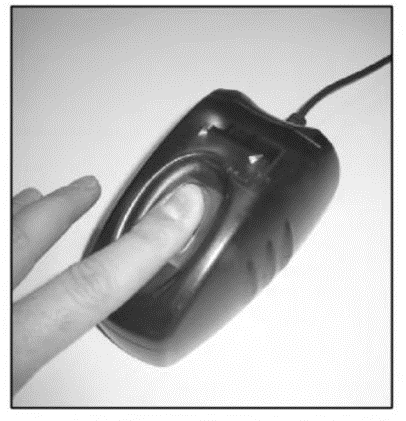
\includegraphics[height=0.45\textwidth]{img/chapter_br/fingerprint_equip.png}}
\subfigure[指纹图像]{
\label{fig:fingerprint_img}
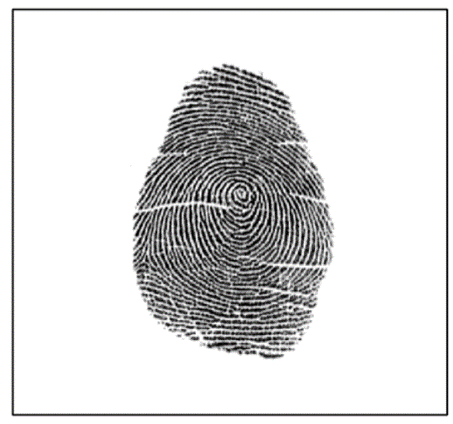
\includegraphics[height=0.45\textwidth]{img/chapter_br/fingerprint_img.png}}
\caption{指纹采集设备和图像\cite{maltoni2009handbook}}
\label{fig:fingerprint}
\end{figure}

掌纹识别是近些年提出的一种相对较新的生物特征识别技术。掌纹一般指手指末端到手腕之间这一区域的手掌表面的各种纹理特征,如图\ref{fig:palmprint_img}所示。与指纹识别类似,每个人的掌纹纹理都不一样,掌纹中具有的很多特征可以进行测量并提取特征值,进而进行身份认证。指纹识别和掌纹识别都是非侵犯性的识别方法,实际应用中用户接受度较高。

\begin{figure}[ht]
\centering  %图片全局居中
\subfigure[掌纹采集设备]{
\label{fig:palmprint_equip}
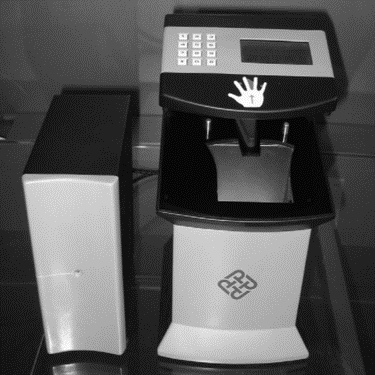
\includegraphics[height=0.45\textwidth]{img/chapter_br/palmprint_equip.png}}
\subfigure[掌纹图像]{
\label{fig:palmprint_img}
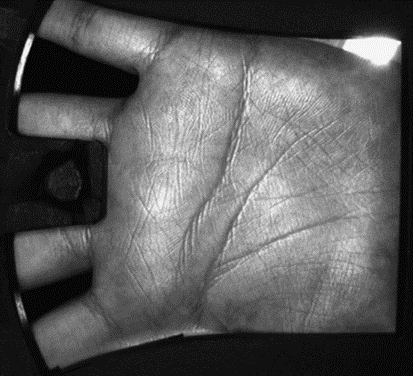
\includegraphics[height=0.45\textwidth]{img/chapter_br/palmprint_img.png}}
\caption{掌纹采集设备和图像\cite{kong2009survey}}
\label{fig:palmprint}
\end{figure}

\section{静脉识别}
静脉识别利用的是静脉中的血红蛋白相对于肌肉、骨骼等其他生理组织对近红外光的吸收率更高,当有近红外光照射在手指或者手掌上时,通过红外摄像头获取手指或手掌的图像,静脉血管会呈现深色,肌肉组织则为浅色,呈现出黑白对比分明的图像特点,如图\ref{fig:finger_vein}所示,静脉血管结构可以清晰的得到呈现。静脉识别技术通过算法对图像进行分析,提取特征值进行身份认证。静脉采集设备按照近红外光源和图像传感器的相对位置不同,主要分为透射式和反射式两种,如图\ref{fig:finger_vein_equip}所示。

\begin{figure}[ht]
\centering  %图片全局居中
\subfigure[指静脉反射式成像]{
\label{fig:finger_vein_1}
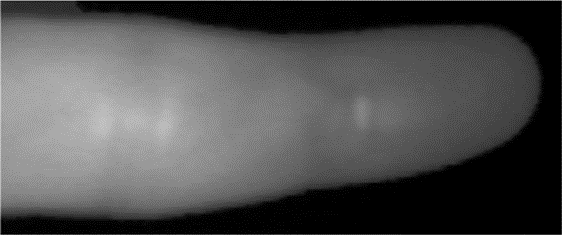
\includegraphics[width=0.65\textwidth]{img/chapter_br/finger_vein.png}}
\subfigure[指静脉透射式成像]{
\label{fig:finger_vein_2}
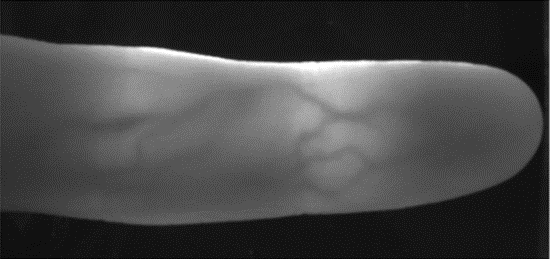
\includegraphics[width=0.65\textwidth]{img/chapter_br/finger_vein_2.png}}
\caption{指静脉图像\cite{hashimoto2006finger}}
\label{fig:finger_vein}
\end{figure}

\begin{figure}[ht]
\centering
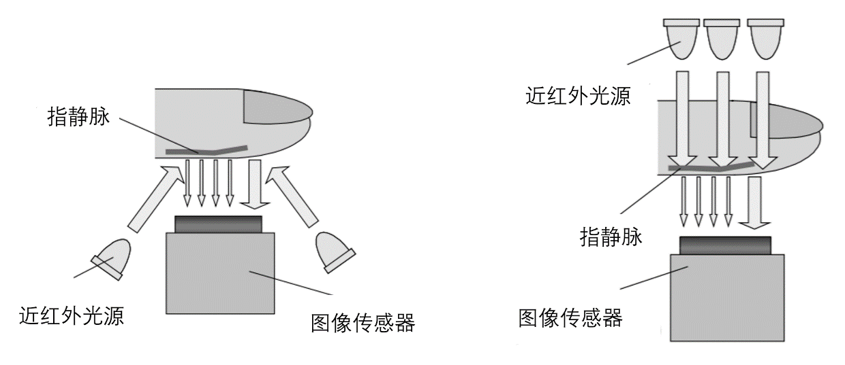
\includegraphics[scale=0.6]{img/chapter_br/finger_vein_equip.png}
\caption{两种指静脉图像采集方式示意图\cite{hashimoto2006finger}}
\label{fig:finger_vein_equip}
\end{figure}

由于静脉属于人体内部特征,相比人脸和指纹来说极难复制和盗取,且只有在活体上才能采集到,因此这项技术的安全性更好,更难以被盗取和假冒。静脉识别过程中一般受外界环境因素(例如温度、湿度等)以及个体皮肤表面状态(如粗糙程度、是否磨损等)影响较小,可靠性较高。同时在使用过程中,用户手无需与设备进行接触,这种非接触式的使用更加卫生、易于用户接受。目前静脉识别技术发展时间较短,识别准确率有望进一步得到提升。由于在活体鉴定方面的优势,与指纹融合可以较好地预防假指纹攻击,并提高识别准确率。
静脉识别在金融行业的应用也已开始了探索。2016年1月,工农中建四大银行委托广电运通起草指静脉在金融行业的应用标准。2016年11月,广东省社保基金管理局也已经制定指静脉在社保行业的应用标准,计划全省开始推广指静脉养老金发放的认证工作。

\section{虹膜识别}

虹膜是位于人眼表面黑色瞳孔和白色巩膜之间的圆环状区域,在近红外光下能够呈现出丰富的纹理,如图\ref{fig:iris_img}所示。而且虹膜在胎儿发育阶段形成后的整个生命历程中是保持不变的。这些特征决定的虹膜特征以及用于身份识别的唯一性。虹膜识别属于非接触式识别,通过专门的虹膜图像采集装置采集清晰的虹膜图像提取特征进行身份认证,识别过程高效且准确率高。虹膜识别技术被认为是生物特征识别技术中准确率最高的技术之一,在金融领域一般应用于金库管理、押运管理的较多,通过虹膜识别确认出入和押运人员身份,确保财产安全;同时,也有部分银行在尝试将虹膜识别和指静脉识别集成于自助终端中,实现更高安全级别的身份认证,以帮助用户完成自助贷款、自助理财等业务的办理。在其他行业,虹膜识别技术因眼镜、光线干扰和特征部位与采集方式等因素,目前主要用于煤矿工人等其他种类生物特征难以采集和识别的人群。

\begin{figure}[ht]
\centering
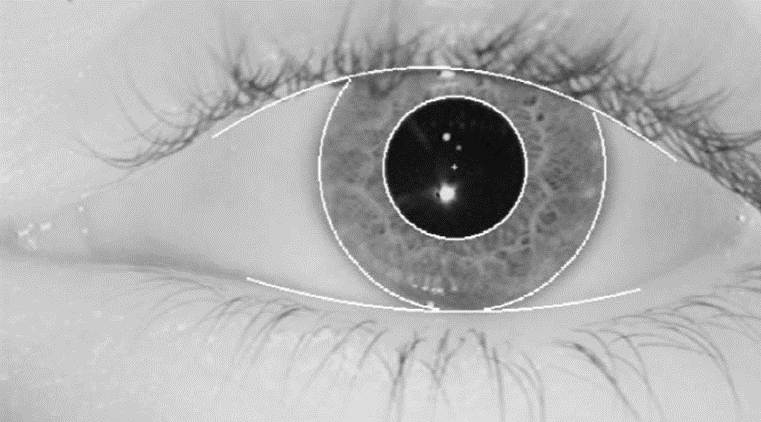
\includegraphics[scale=0.6]{img/chapter_br/iris_img.png}
\caption{虹膜图像\cite{daugman2009iris}}
\label{fig:iris_img}
\end{figure}

以上是目前较为常见的几种生物特征识别技术。随着智能终端设备以及生物特征传感器的快速普及和优化,生物特征识别技术已经进入大规模应用阶段。单一的人脸识别或指纹识别已经难以满足金融机构的多样化需求,多模态生物识别是金融科技不可更改的趋势。
%%%%%%%%%%%%%%%%%%%%% chapter.tex %%%%%%%%%%%%%%%%%%%%%%%%%%%%%%%%%
%
% sample chapter
%
% Use this file as a template for your own input.
%
%%%%%%%%%%%%%%%%%%%%%%%% Springer-Verlag %%%%%%%%%%%%%%%%%%%%%%%%%%
%\motto{Use the template \emph{chapter.tex} to style the various elements of your chapter content.}
\chapter{反欺诈:声纹与人脸识别的抗攻击}
\label{basic} % Always give a unique label
% use \chaptermark{}
% to alter or adjust the chapter heading in the running head


这是里关于主题模型和语言模型的介绍。

\section{声纹识别中的抗攻击}

随着声纹识别的应用越来越广泛,声纹识别的安全性要求也越来越高。因此声纹识别研究中,必须了解声纹识别的攻击技术,才能进一步进行防范。在声纹识别应用中,主要的攻击方法分为四大类:模拟(Impersonation)、录播(Replay)、语音合成(Speech Synthesis)和语音转换(Voice Conversion)。

模拟攻击通常来自两种情况:双胞胎和专业模仿人员。双胞胎主要是因为生物信息相对比较接近,所以存在声纹接近的可能。曾经有报道说有双胞胎弟弟用自己声音破解了哥哥在银行的声纹密码。有论文~\cite{patil2005speaker}提到这个问题,从他们的实验结果来看,就算是双胞胎还是存在一定的差异性,能进行区分。对应专业模仿人员,也有数据~\cite{patil2008lp}显示具有声纹攻击性,但是差异比双胞胎大。这一类攻击最大的问题就是可供训练和测试的数据很有限,小数据上能进行防范,但是对于其真正的攻击情况目前认为是不确定的。

录播攻击,一般是用录音机对特定人进行录音,然后播放出来从而达到声纹认证通过的效果。在ASVspoof2017~\cite{kinnunen2017asvspoof}比赛中,通过参赛人的比赛结果以及对往届的比赛结果来看,录播攻击识别难度比语音合成、语音转换攻击识别难度更高。录播攻击其中涉及到录音环境、播放环境、录音设备等干扰,会一定程度对识别是否是攻击造成一定难度。

语音合成攻击,一般分为两类,一个是拼接方式,一个是TTS语音生成方式。针对TTS,机器识别准确一般比较高,因此不会造成比较大的威胁。但是语音拼接,这种技术方式,针对我们人耳能准确识别,但是对于机器而已,他们比较大可能认为是真实说话声音。

语音转换是把一个人说话的录音改变音色,频率等转换为具有另外一个人说话特点的技术~\cite{jia2018transfer}。一般会用语音转换和TTS技术进行结合进行攻击,这样能比较方便有效,相对攻击成本比较低。这种攻击方式通常都能识别出来,机器生成的毕竟存在一定模式规律。但是也会存在一种风险,这种防止攻击的鲁棒性不一定很高。

针对这一系列的攻击方法,通用的抗攻击框架是在声纹识别前增加一个前置模块,用来专门识别是否是攻击。目前业界对这些攻击方式能较为准确识别,但是需要不断积累足够大的样本,从而提高更高的防护能力。


\section{人脸识别中的抗攻击}

人脸活体检测( Face Anti-Spoofing)技术是人脸识别系统中,用以确认待认证对象是否为真实生物活体的一项技术。一方面,人脸识别技术的商业化愈加成熟和广泛,极大改善和推进了社会金融活动的智能化和便捷性;另一方面,由于人脸照片、视频数据相对容易获取和复制,若无活体检测这一环节,那么使用被盗取的合法用户的照片、视频或者3D面及头套等即可入侵人脸识别系统,由此将带来极大危害\cite{chingovska2012effectiveness}。在目前的人脸识别系统中,常见的活体检测技术包括动作活体、3D活体、红外活体、光线活体等。下面将逐一简单介绍。

动作活体是通过利用人脸关键点和人脸跟踪等技术,检测用户眨眼、张嘴、摇头等多种动作及其组合,可有效抵御照片、换脸、面具、遮挡以及屏幕翻拍等常见的攻击手段,但较难抵御视频回放攻击。

3D活体通过专用硬件(例如3D结构光、ToF等)获取人脸部3D结构信息,可以有效防御如手机、电脑等屏幕显示和打印照片等2D攻击手段,但是需要配合其他方法抵御近几年出现的高质量3D面具攻击\cite{zhang2019dataset}。

红外活体检测一般利用人体皮肤对近红外光的反射率较高,相比于其他材质有明显区别的特性,通过专用红外设备获取人脸部红外图像判断是否为活体。实际应用中通常使用主动红外摄像,即通过红外LED照射人脸,利用红外摄像头获取人脸部图像,分类判断是否为活体。红外活体检测技术对于常见攻击手段具有较好的防御效果,缺点在于需要特定红外设备\cite{zhang2019dataset,yi2014face}。

光线活体是近两年出现的一种活体检测技术。由于3D活体、红外活体需要特殊设备,在已有系统中部署较为困难。光线活体技术利用屏幕发出不同颜色和强度的光线照射在人脸上,由于人脸自身的三维结构以及皮肤等生理组织对于不同颜色光线的反射率不同,从获取的视频中提取相应的活体信息,如图\ref{fig:light_reflection}所示。这项技术由于无需特殊硬件设备、且具有较高的准确率,在手机等移动端使用较为方便。其缺点在于要求视频拍摄过程稳定,闪光带来的用户体验需要得到提升,同时户外强光也会带来较大干扰\cite{liu2019aurora}。

\begin{figure}[ht]
\centering
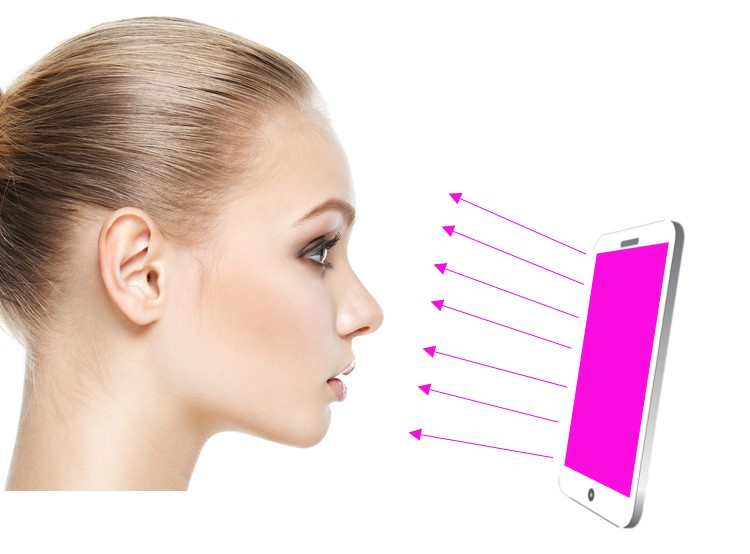
\includegraphics[scale=0.5]{img/chapter_as/light_reflection.jpg}
\caption{光线活体}
\label{fig:light_reflection}
\end{figure}

\bibliographystyle{gbt7714-2005}
\bibliography{chapters/reference}

\backmatter%%%%%%%%%%%%%%%%%%%%%%%%%%%%%%%%%%%%%%%%%%%%%%%%%%%%%%%
%\include{glossary}
%\include{solutions}
\printindex

%%%%%%%%%%%%%%%%%%%%%%%%%%%%%%%%%%%%%%%%%%%%%%%%%%%%%%%%%%%%%%%%%%%%%%

\end{document}





